\documentclass{article}
\usepackage[margin=1in]{geometry}
\usepackage[utf8]{inputenc}
\usepackage{amsfonts,amsmath,bm}
\usepackage{xcolor}
\usepackage{graphicx}
\usepackage{caption}
\usepackage{subcaption}
\usepackage{tabulary}
\usepackage{multirow}
\usepackage{algorithm}
\usepackage{algpseudocode}
\usepackage{hyperref}
% color def
\usepackage{color}
\definecolor{darkred}{rgb}{0.6,0.0,0.0}
\definecolor{darkgreen}{rgb}{0,0.50,0}
\definecolor{lightblue}{rgb}{0.0,0.42,0.91}
\definecolor{orange}{rgb}{0.99,0.48,0.13}
\definecolor{grass}{rgb}{0.18,0.80,0.18}
\definecolor{pink}{rgb}{0.97,0.15,0.45}

% listings
\usepackage{listings}

% General Setting of listings
\lstset{
  aboveskip=1em,
  breaklines=true,
  abovecaptionskip=-6pt,
  captionpos=b,
  escapeinside={\%*}{*)},
  frame=single,
  numbers=left,
  numbersep=15pt,
  numberstyle=\tiny,
}
% 0. Basic Color Theme
\lstdefinestyle{colored}{ %
  basicstyle=\ttfamily,
  backgroundcolor=\color{white},
  commentstyle=\color{green}\itshape,
  keywordstyle=\color{blue}\bfseries\itshape,
  stringstyle=\color{red},
}
% 1. General Python Keywords List
\lstdefinelanguage{PythonPlus}[]{Python}{
  morekeywords=[1]{,as,assert,nonlocal,with,yield,self,True,False,None,} % Python builtin
  morekeywords=[2]{,__init__,__add__,__mul__,__div__,__sub__,__call__,__getitem__,__setitem__,__eq__,__ne__,__nonzero__,__rmul__,__radd__,__repr__,__str__,__get__,__truediv__,__pow__,__name__,__future__,__all__,}, % magic methods
  morekeywords=[3]{,object,type,isinstance,copy,deepcopy,zip,enumerate,reversed,list,set,len,dict,tuple,range,xrange,append,execfile,real,imag,reduce,str,repr,}, % common functions
  morekeywords=[4]{,Exception,NameError,IndexError,SyntaxError,TypeError,ValueError,OverflowError,ZeroDivisionError,}, % errors
  morekeywords=[5]{,ode,fsolve,sqrt,exp,sin,cos,arctan,arctan2,arccos,pi, array,norm,solve,dot,arange,isscalar,max,sum,flatten,shape,reshape,find,any,all,abs,plot,linspace,legend,quad,polyval,polyfit,hstack,concatenate,vstack,column_stack,empty,zeros,ones,rand,vander,grid,pcolor,eig,eigs,eigvals,svd,qr,tan,det,logspace,roll,min,mean,cumsum,cumprod,diff,vectorize,lstsq,cla,eye,xlabel,ylabel,squeeze,}, % numpy / math
}
% 2. New Language based on Python
\lstdefinelanguage{PyBrIM}[]{PythonPlus}{
  emph={d,E,a,Fc28,Fy,Fu,D,des,supplier,Material,Rectangle,PyElmt},
}
% 3. Extended theme
\lstdefinestyle{colorEX}{
  basicstyle=\ttfamily,
  backgroundcolor=\color{white},
  commentstyle=\color{darkgreen}\slshape,
  keywordstyle=\color{blue}\bfseries\itshape,
  keywordstyle=[2]\color{blue}\bfseries,
  keywordstyle=[3]\color{grass},
  keywordstyle=[4]\color{red},
  keywordstyle=[5]\color{orange},
  stringstyle=\color{darkred},
  emphstyle=\color{pink}\underbar,
}
% \usepackage{biblatex}
% \addbibresource{bibliography.bib} %Import the bibliography file
% \usepackage[framed,numbered,autolinebreaks,useliterate]{mcode}
\usepackage{tikz}
\newcommand*\circled[1]{\tikz[baseline= (char.base)]{
            \node[shape=circle, draw, inner sep=1.5pt] (char) {#1};}}
\newcommand*\smallcircled[1]{\tikz[baseline= (char.base)]{
            \node[shape=circle, draw, inner sep=0.5pt] (char) {#1};}}


\title{EEC269A - Error Correcting Codes I\\Project Report}
\author{Chenye Yang, Pranav Kharche, Parisa Oftadeh}
\date{\today}

\begin{document}

\maketitle

\tableofcontents














\newpage
\section{Workload}

\begin{table}[htb]
    \centering
    \caption{Workload}
    \label{tab:workload}
    \renewcommand{\arraystretch}{1.5}
    \begin{tabulary}{\textwidth}{ |L|L|L| } 
    \hline
    \textbf{Function} & \textbf{Workload} & \textbf{Contributor} \\
    \hline
    Source & Text string (TXT), Image (PNG), Audio (WAV) & Chenye \\ 
    \hline
    \multirow{2}{*}{Encoder} & $(7,4)$ Systematic Linear Block (Hamming) Code & Chenye \\ 
    & $(n,k)$ Systematic Cyclic (Hamming) Code & Pranav, Chenye \\ 
    \hline
    \multirow{1}{*}{Channel} & Binary Symmetric Channel (BSC), error probability $p$ adjustable & Chenye \\ 
    \hline
    \multirow{3}{*}{Error Corrector} &  Syndrome Lookup Table for $(7,4)$ Linear Code & Chenye \\ 
    & Syndrome Lookup Table for $(n,k)$ Cyclic Code & Chenye \\ 
    & LFSR for $(n,k)$ Cyclic Code & \textcolor{red}{TODO} \\
    \hline
    \multirow{2}{*}{Decoder} & $(7,4)$ Systematic Linear Block (Hamming) Code & Chenye \\ 
    & $(n,k)$ Systematic Cyclic (Hamming) Code & Chenye \\ 
    \hline
    Destination & Text string (TXT), Image (PNG), Audio (WAV) & Chenye \\ 
    \hline
    \multirow{2}{*}{\textbf{Advanced}} & \textbf{Create generator matrix for $(n,k)$ cyclic code} & Pranav \\ 
    & \textbf{Adjustable $(n,k)$} & Pranav \\ 
    \hline
    \end{tabulary}
\end{table}



\section{Source \& Destination}
\subsection{Source}

\subsubsection{Text string}
The very basic function of the information source is to read a hard-coded text file into a bit stream. 
In our text file, the following string is stored in ASCII format:
\begin{center}
    Hello World!\\EEC269A Error Correcting Code Demo
\end{center}
In ASCII format, each character is represented by 8 bits, shown in Table~\ref{tab:ascii}. Then, after transformation, the bit stream is of size 376 bits: 
\begin{center}
    0 1 0 0 1 0 0 0 0 1 1 0 0 1 0 1 \dots
\end{center}

\begin{table}[ht]
    \centering
    \caption{ASCII Table example}
    \label{tab:ascii}
    \begin{tabulary}{\textwidth}{|L|L|L|L|}
    \hline
    Character & Hexadecimal & Decimal & Binary \\
    \hline
    \dots & \dots & \dots & \dots \\
    \hline
    A & 41 & 65 & 0 1 0 0 0 0 0 1 \\
    \hline
    B & 42 & 66 & 0 1 0 0 0 0 1 0 \\
    \hline
    C & 43 & 67 & 0 1 0 0 0 0 1 1 \\
    \hline
    D & 44 & 68 & 0 1 0 0 0 1 0 0 \\
    \hline
    E & 45 & 69 & 0 1 0 0 0 1 0 1 \\
    \hline
    F & 46 & 70 & 0 1 0 0 0 1 1 0 \\
    \hline
    G & 47 & 71 & 0 1 0 0 0 1 1 1 \\
    \hline
    H & 48 & 72 & 0 1 0 0 1 0 0 0 \\
    \hline
    \dots & \dots & \dots & \dots \\
    \hline
    \end{tabulary}
\end{table}


\subsubsection{Image}
A PNG file is composed of an 8-byte signature header, followed by any number of chunks that contain control data / metadata / image data. 
Each chunk contains three standard fields: 4-byte length, 4-byte type code, 4-byte CRC and various internal fields that depend on the chunk type, shown in Figure~\ref{fig:png-structure}. 
For example, the image file we are using has more than one image data (IDAT) chunks, each of which contains a portion of the image, shown in Table~\ref{tab:our-png-structure}.

Ideally, the entire image file should be read into a bit stream and transmitted through the channel. 
However, if there are uncorrectable errors in the chunks other than the image data (IDAT), the received image will not be able to display.
Therefore, we shall only work with the image data (IDAT) chunks for the purpose of visualization of a corrupted image.

The information source is able to only extract the color information from a PNG file and convert it into a bit stream to be passed through the channel. 
This is done by using the Python library \textit{numpy}.

The library \textit{numpy} provides a method to only read out the color information of an image. The shape of the result array is typically \textit{(height, width, channels)}, where:
\begin{enumerate}
    \item \textit{height} is the number of pixels in the vertical direction (i.e. the number of rows of pixels);
    \item \textit{width} is the number of pixels in the horizontal direction (i.e. the number of columns of pixels);
    \item \textit{channels} is the number of color channels per pixel. This value depends on what type of image it is: \begin{itemize}
        \item In an RGB image, the three channels correspond to Red, Green, and Blue, respectively. Each channel value usually ranges from 0 to 255, where 0 indicates none of that color is present and 255 indicates that color is fully present.
        \item In a grayscale image, there is typically only one channel. The value in this single channel indicates the level of gray, where 0 is black and 255 is white.
        \item There are many other color spaces (HSV, LAB, etc.) that have different meanings for their channels.
    \end{itemize}
\end{enumerate}
The data type for each channel of each pixel is \textit{uint8}, which is an unsigned integer that takes 8 bits.
Then, the array is flattened into a bit stream by converting each channel of each pixel into an 8-bits binary number and appending them together.

For example, as for our testing image\footnote{The image file '\textit{image.png}' used in this project is photographed by \textit{Chenye Yang} at Joshua Tree National Park.}, shown in Figure~\ref{fig:our-image}, the shape of the result array is \textit{(1280, 854, 3)}, which means that the image has 1280 rows of pixels, 854 columns of pixels, and 3 color channels per pixel (RGB). 
Then, the array is flattened into a bit stream of 26,234,880 bits.


\begin{figure}[htb]
    \centering
    \hfill
    \begin{minipage}[b]{0.3\textwidth}
        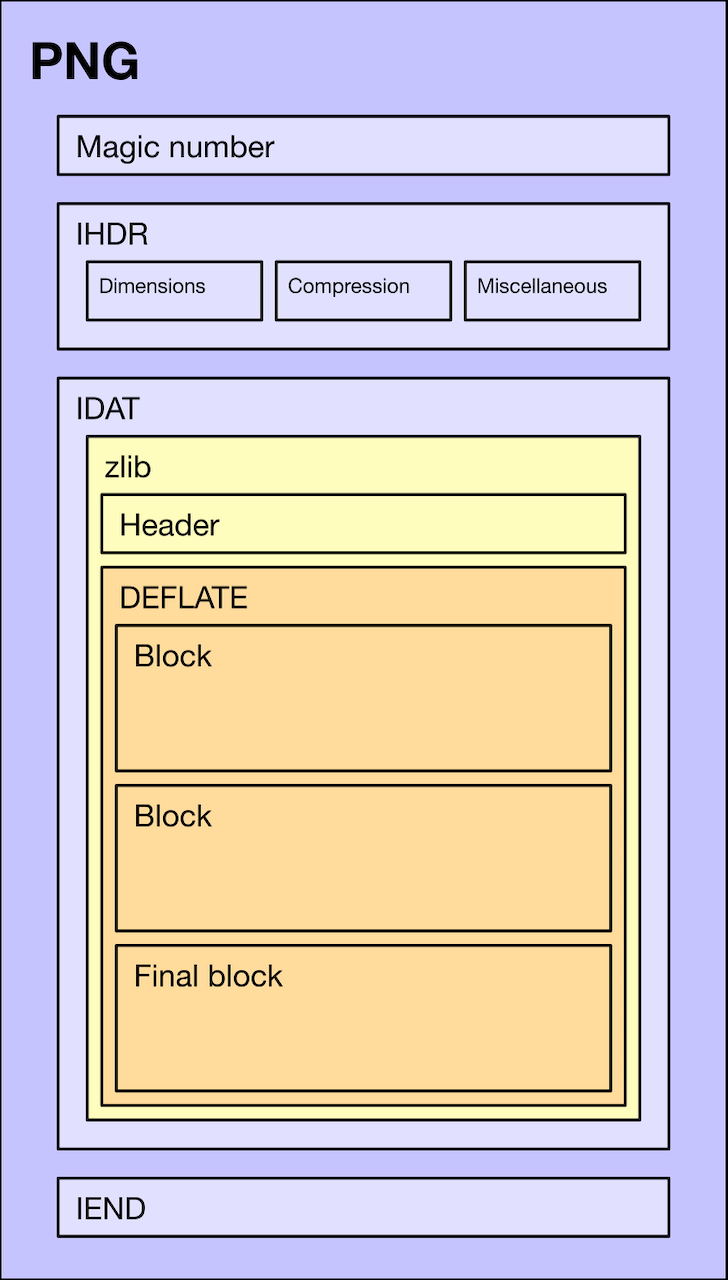
\includegraphics[width=\textwidth]{png-file-format.png}
        \caption{PNG file structure}
    \label{fig:png-structure}
    \end{minipage}
    \hfill
    \begin{minipage}[b]{0.36\textwidth}
        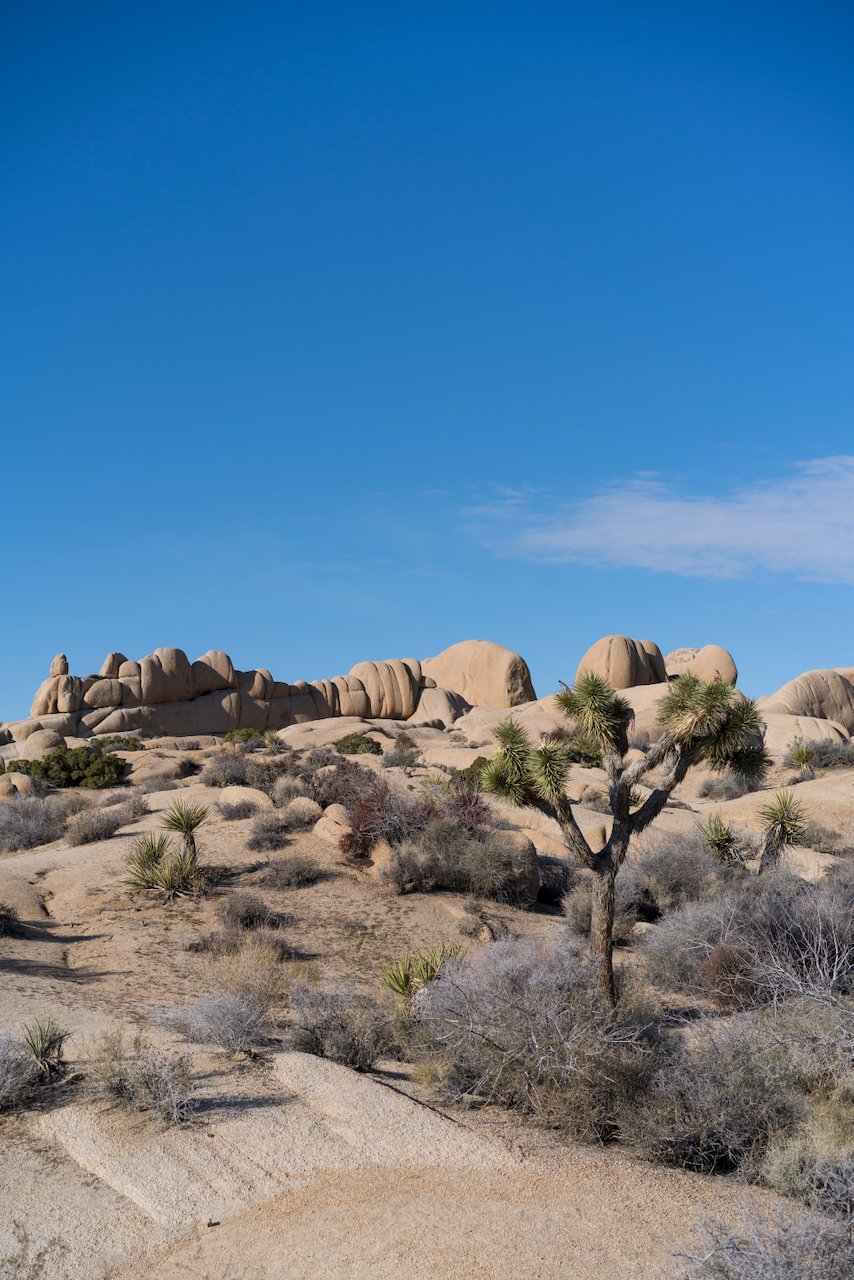
\includegraphics[width=\textwidth]{../Resource/image.png}
        \caption{Our testing PNG image}
    \label{fig:our-image}
    \end{minipage}
    \hfill
\end{figure}



\begin{table}[htb]
    \centering
    \caption{Our PNG file structure}
    \label{tab:our-png-structure}
    \renewcommand{\arraystretch}{1.5}
    \begin{tabulary}{\textwidth}{ |L|L| } 
    \hline
    Start offset & Chunk outside \\
    \hline
    0 & Special: File signature; Length: 8 bytes \\
    \hline
    8 & Data length: 13 bytes; Type: IHDR; Name: Image header; CRC-32: CB3954EC \\
    \hline
    33 & Data length: 1 bytes; Type: sRGB; Name: Standard RGB color space; CRC-32: AECE1CE9 \\
    \hline
    46 & Data length: 976 bytes; Type: eXIf; Name: Exchangeable Image File (Exif) Profile; CRC-32: 47FCFA4D \\
    \hline
    1,034 & Data length: 9 bytes; Type: pHYs; Name: Physical pixel dimensions; CRC-32: 5024E7F8 \\
    \hline
    1,055 & Data length: 4 514 bytes; Type: iTXt; Name: International textual data; CRC-32: C9C76B16 \\
    \hline
    5,581 & Data length: 16 384 bytes; Type: IDAT; Name: Image data; CRC-32: 8462CABD \\
    \hline
    21,977 & Data length: 16 384 bytes; Type: IDAT; Name: Image data; CRC-32: 2C9D007C \\
    \hline
    \dots & \dots \\
    \hline
    1,727,161 & Data length: 12 170 bytes; Type: IDAT; Name: Image data; CRC-32: 68067F52 \\
    \hline
    1,739,343 & Data length: 0 bytes; Type: IEND; Name: Image trailer; CRC-32: AE426082 \\
    \hline
    \end{tabulary}
\end{table}




\subsubsection{Audio}
\footnote{The audio file '\textit{file\_example\_WAV\_1MG.wav}' used in this project is free downloaded from \href{https://file-examples.com/index.php/sample-audio-files/sample-wav-download/}{file-examples.com}.}















\subsection{Destination}





\section{Channel}

\subsection{Binary Symmetric Channel (BSC)}











\subsection{Additive White Gaussian Noise (AWGN) Channel}










\section{(7,4) Systematic Linear Block (Hamming) Code}
\subsection{Syndrome Decoder}
\subsubsection{Text string}

\begin{table}[htb]
    \centering
    \caption{Text string encoded with Linear Hamming passed through BSC}
    \label{tab:text-linear-bsc}
    \renewcommand{\arraystretch}{1.5}
    \begin{tabulary}{\textwidth}{ |L|L|L| } 
    \hline
    \textbf{Original} & \textbf{Without correction} & \textbf{Corrected} \\
    \hline
    Hello World! EEC269A Error Correcting Code Demo & Hello Wo\textcolor{red}{p}ld! EEC269A \textcolor{red}{A}rror Correcting \textcolor{red}{K}ode Demo & Hello World! EEC269A Error Correcting Code Demo \\
    \hline
    \end{tabulary}
\end{table}




\subsubsection{Image}


\begin{figure}[htb]
    \centering
    \begin{subfigure}[b]{0.32\textwidth}
        \centering
        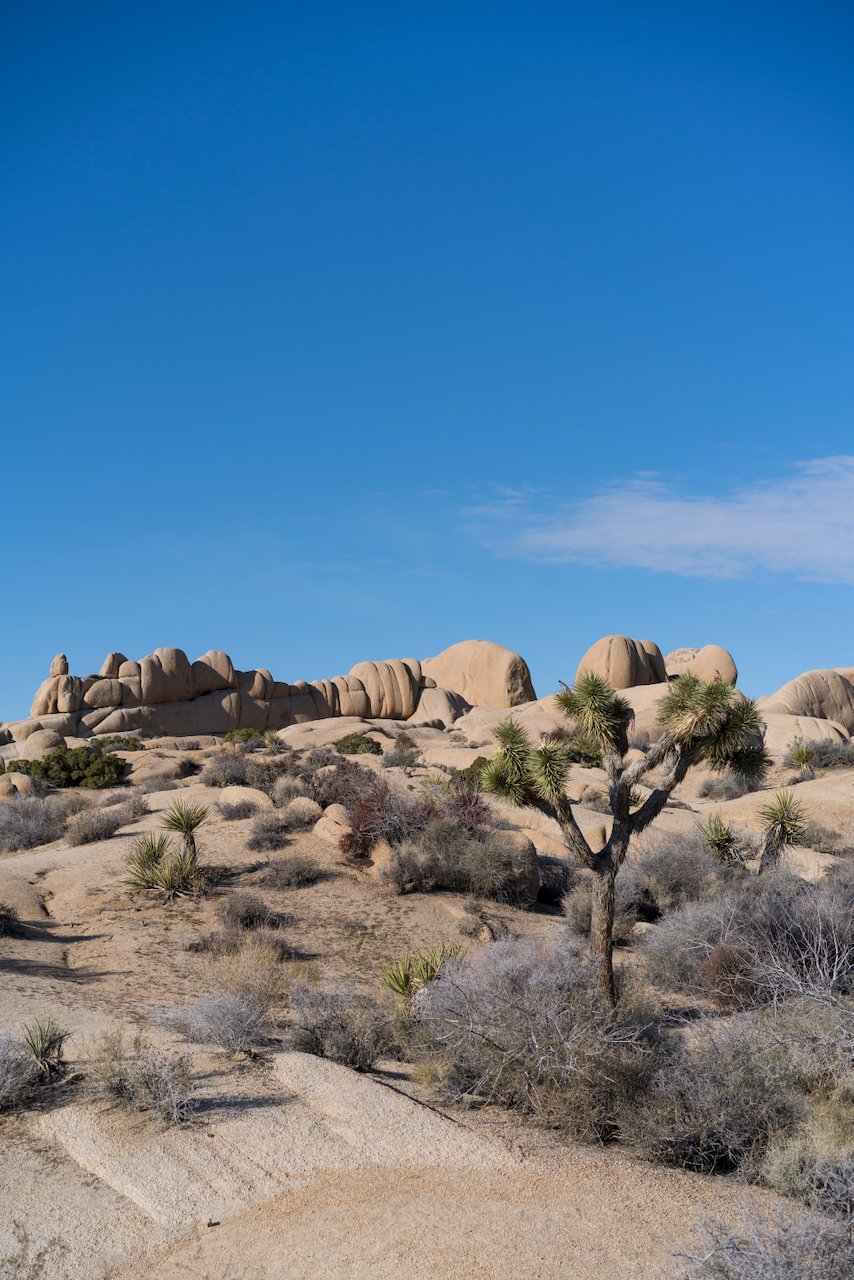
\includegraphics[width=\textwidth]{../Resource/image.png}
        \caption{Original}
        \label{fig:image-linear-bsc-original}
    \end{subfigure}
    \hfill
    \begin{subfigure}[b]{0.32\textwidth}
        \centering
        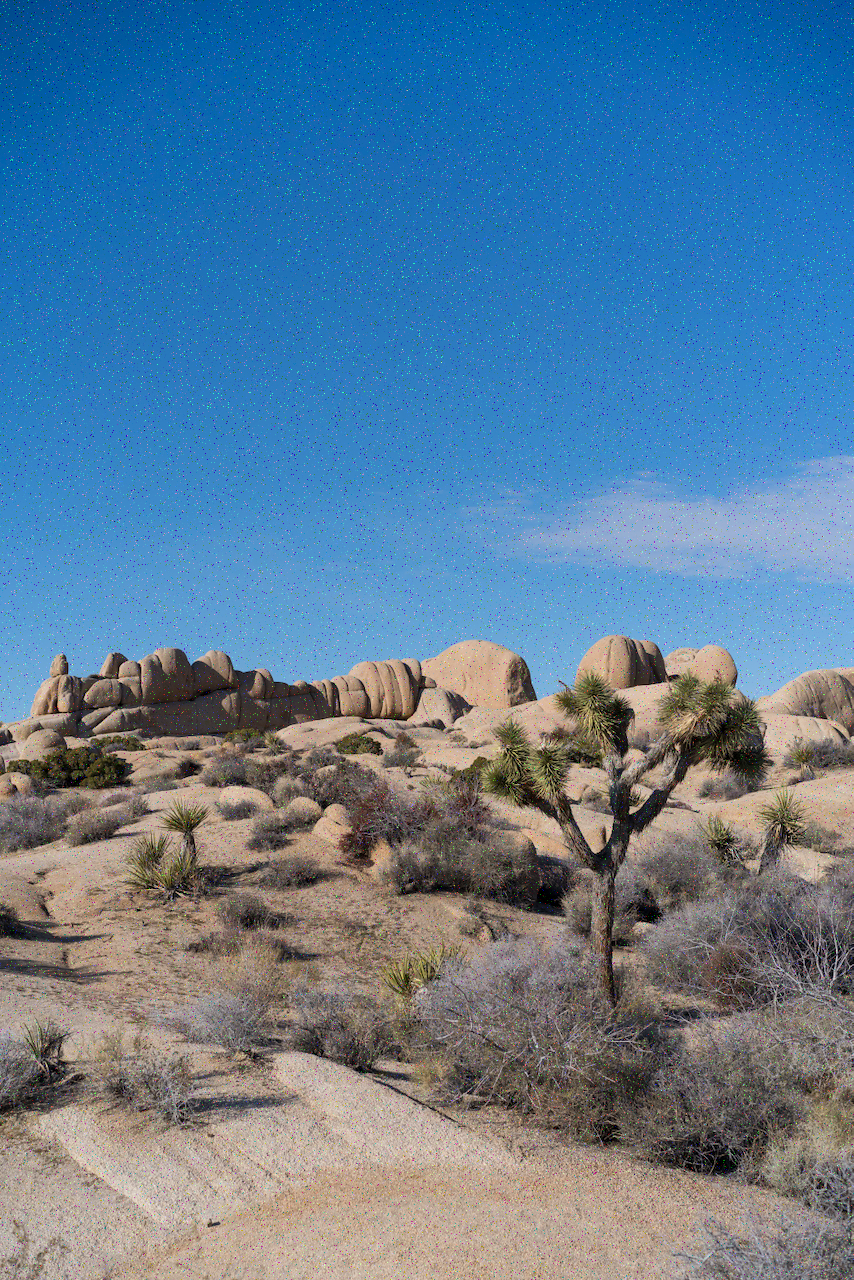
\includegraphics[width=\textwidth]{../Result/linear-bsc-output.png}
        \caption{Without correction}
        \label{fig:image-linear-bsc-no-correction}
    \end{subfigure}
    \hfill
    \begin{subfigure}[b]{0.32\textwidth}
        \centering
        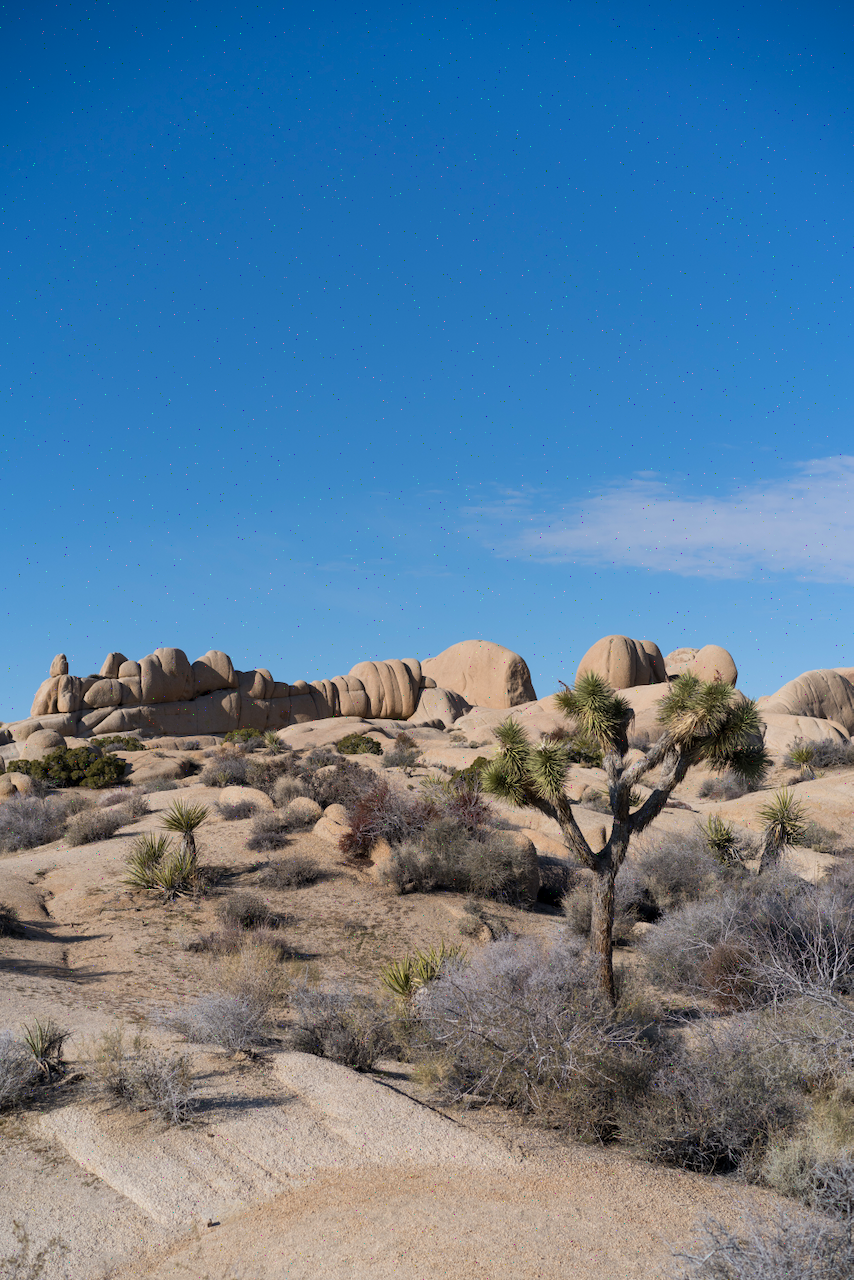
\includegraphics[width=\textwidth]{../Result/linear-bsc-output-syndrome-corrected.png}
        \caption{Corrected}
        \label{fig:image-linear-bsc-syndrome-corrected}
    \end{subfigure}
       \caption{Image encoded with Linear Hamming passed through BSC (entire)}
       \label{fig:image-linear-bsc}
\end{figure}


\begin{figure}[htb]
    \centering
    \begin{subfigure}[b]{0.32\textwidth}
        \centering
        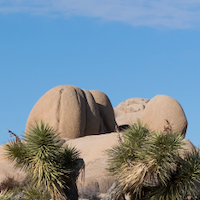
\includegraphics[width=\textwidth]{../Resource/cropped-image.png}
        \caption{Original}
        \label{fig:cropped-image-linear-bsc-original}
    \end{subfigure}
    \hfill
    \begin{subfigure}[b]{0.32\textwidth}
        \centering
        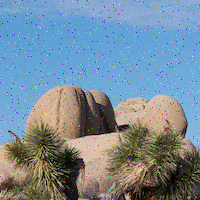
\includegraphics[width=\textwidth]{../Result/cropped-linear-bsc-output.png}
        \caption{Without correction}
        \label{fig:cropped-image-linear-bsc-no-correction}
    \end{subfigure}
    \hfill
    \begin{subfigure}[b]{0.32\textwidth}
        \centering
        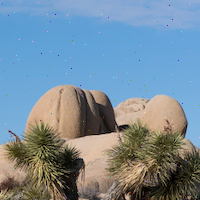
\includegraphics[width=\textwidth]{../Result/cropped-linear-bsc-output-syndrome-corrected.png}
        \caption{Corrected}
        \label{fig:cropped-image-linear-bsc-syndrome-corrected}
    \end{subfigure}
       \caption{Image encoded with Linear Hamming passed through BSC (details)}
       \label{fig:cropped-image-linear-bsc}
\end{figure}


\subsubsection{Audio}


\begin{figure}[htb]
    \centering
    \begin{subfigure}[b]{\textwidth}
        \centering
        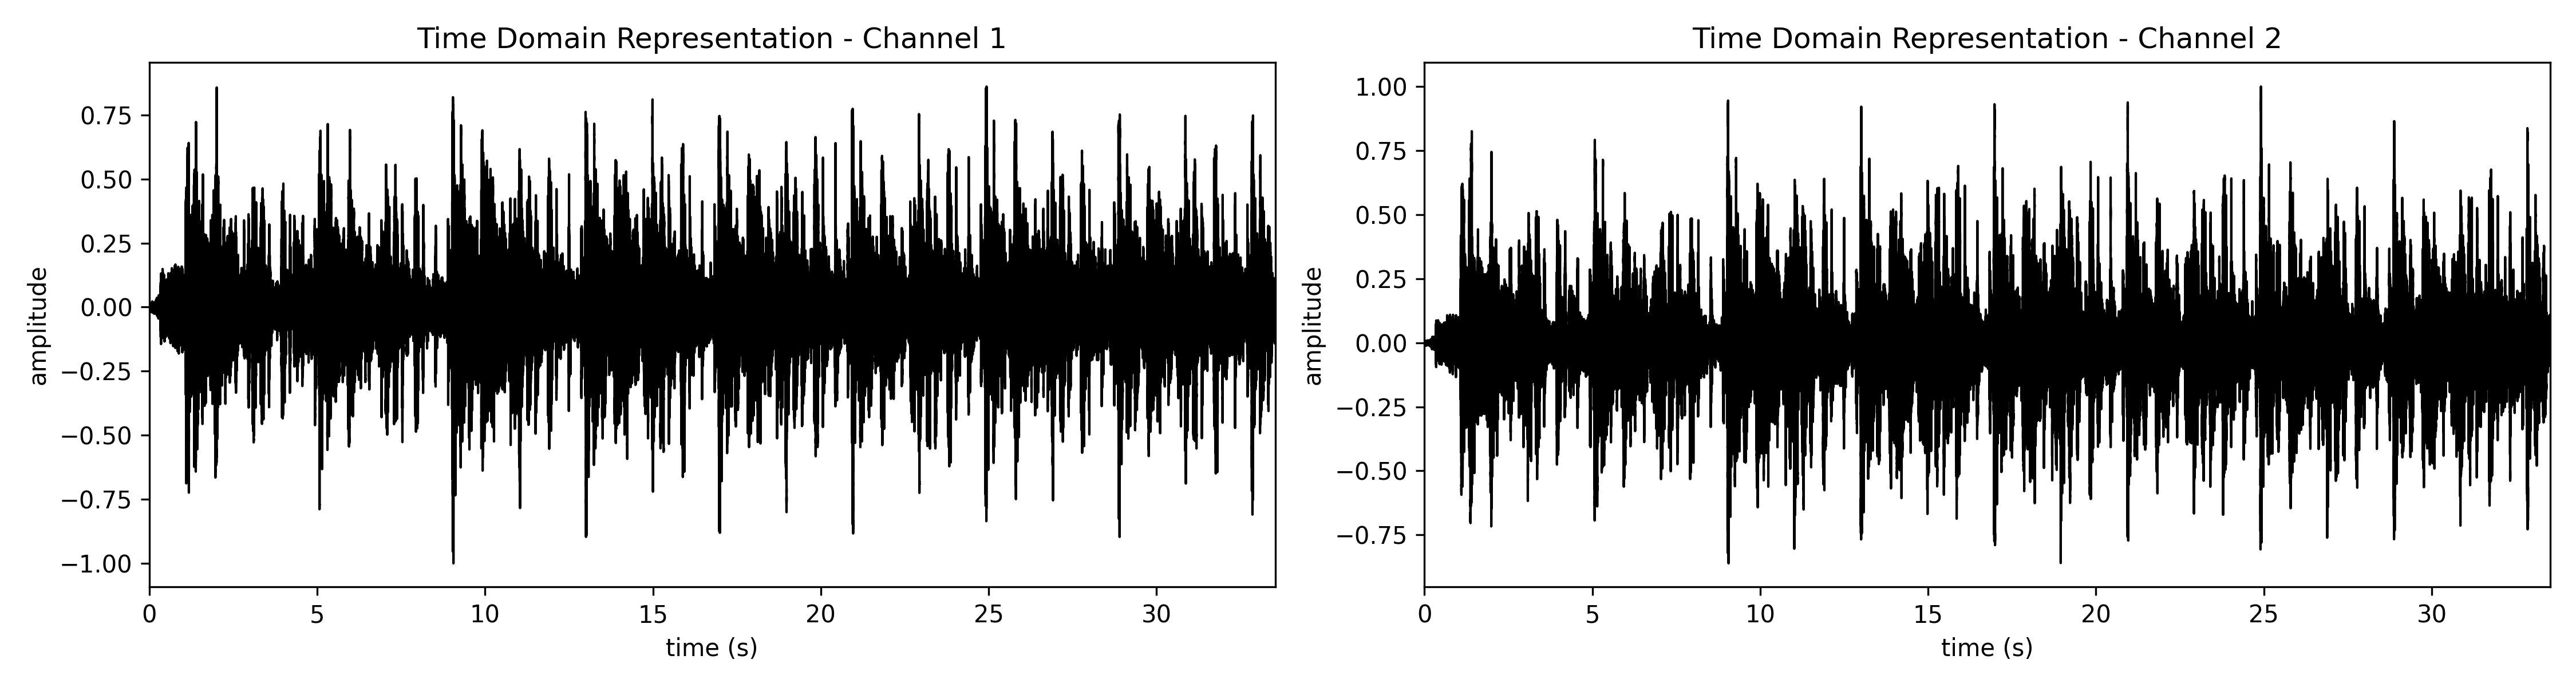
\includegraphics[width=\textwidth]{../Result/wav-time-domain-TX.png}
        \caption{Original}
        \label{fig:t-audio-linear-bsc-original}
    \end{subfigure}
    % \hfill
    \begin{subfigure}[b]{\textwidth}
        \centering
        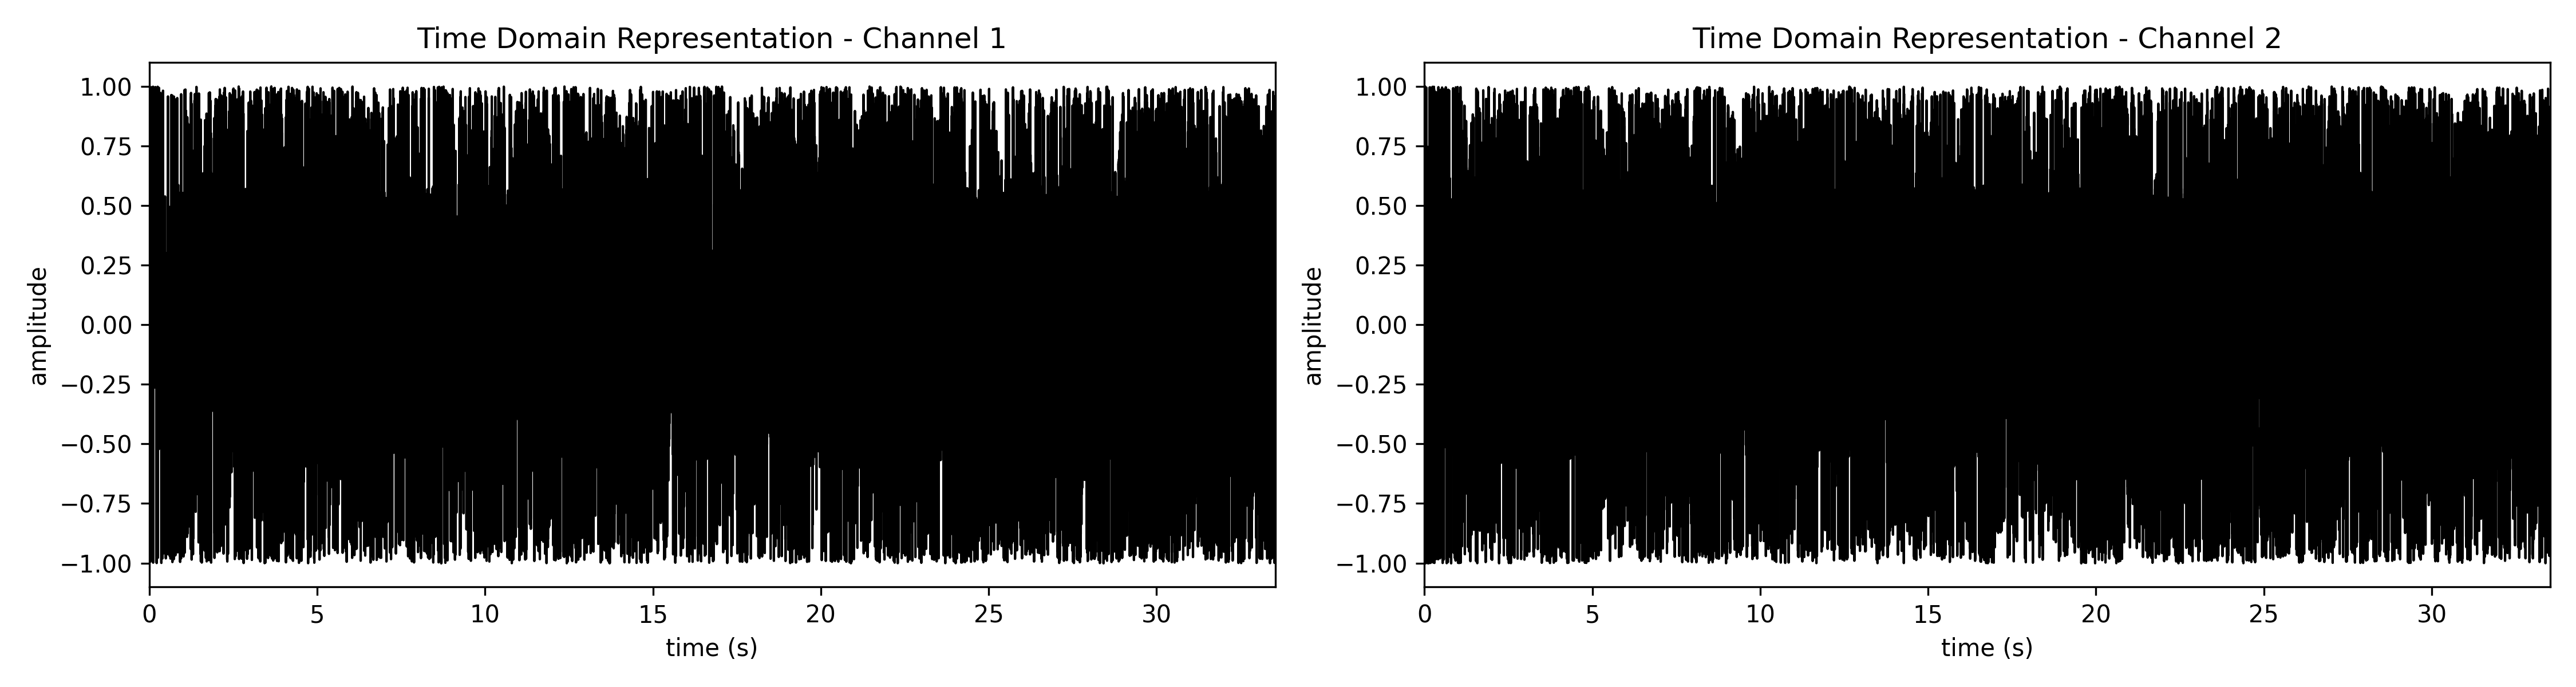
\includegraphics[width=\textwidth]{../Result/linear-bsc-wav-time-domain-RX.png}
        \caption{Without correction}
        \label{fig:t-audio-linear-bsc-no-correction}
    \end{subfigure}
    % \hfill
    \begin{subfigure}[b]{\textwidth}
        \centering
        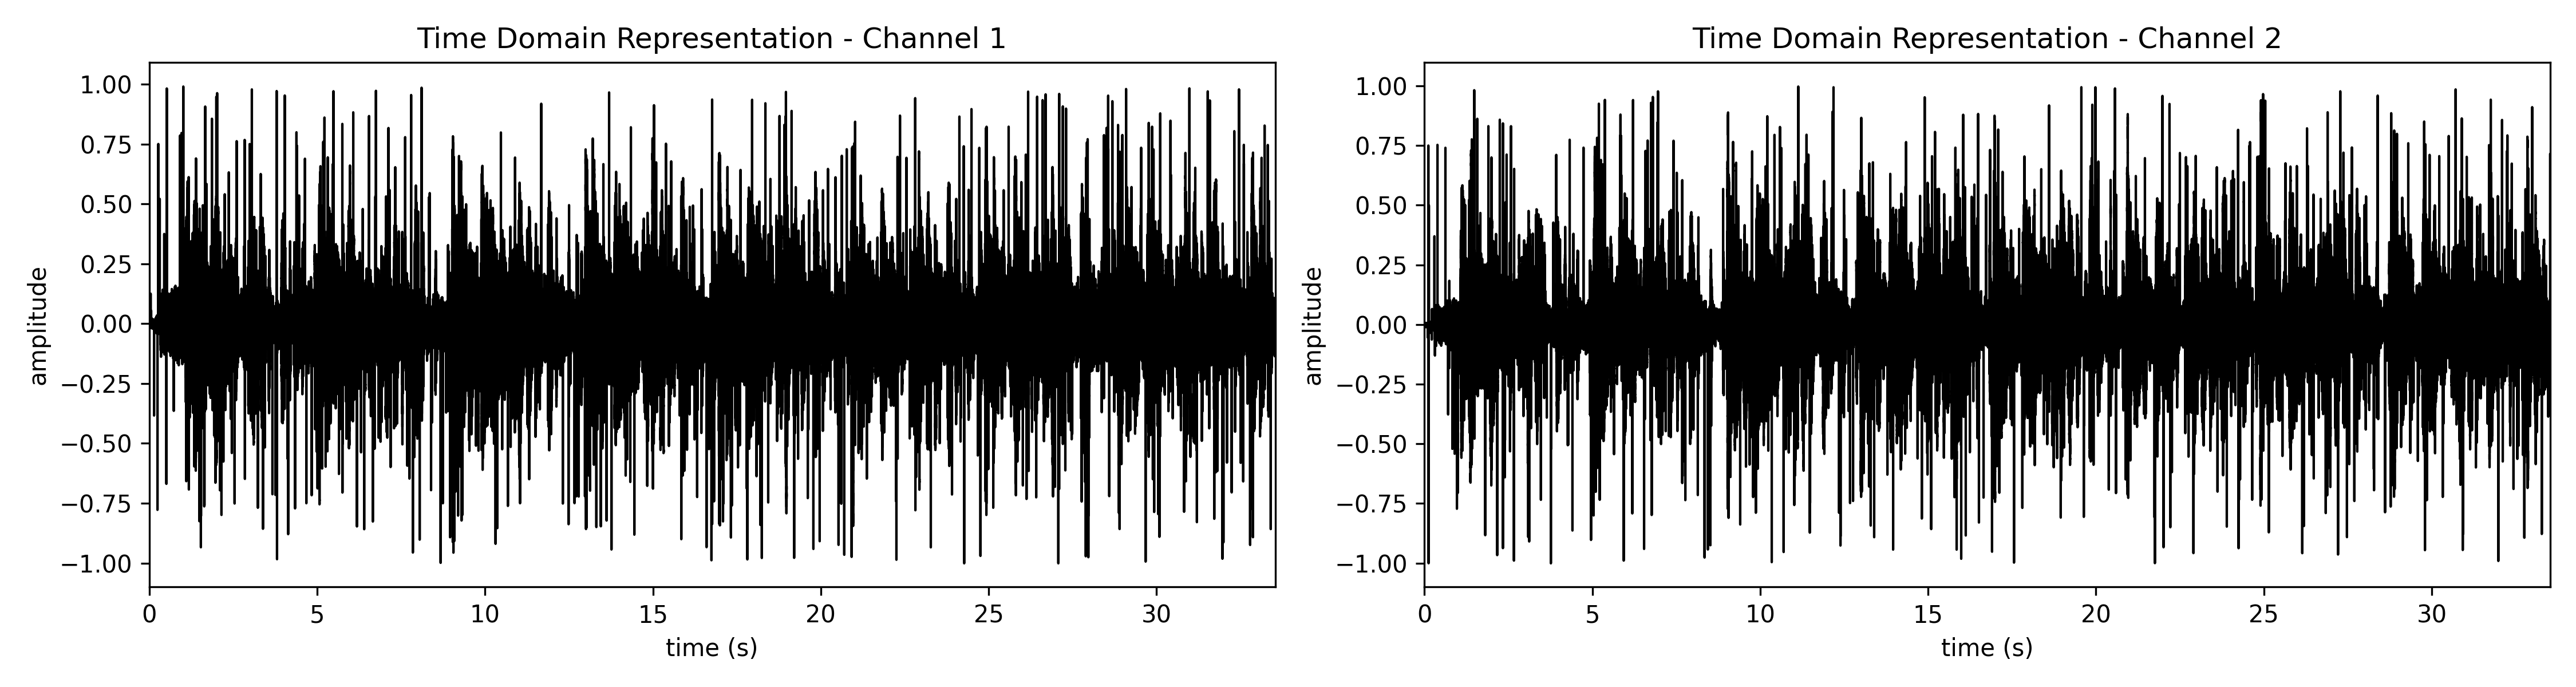
\includegraphics[width=\textwidth]{../Result/linear-bsc-wav-time-domain-RX-syndrome-corrected.png}
        \caption{Corrected}
        \label{fig:t-audio-linear-bsc-syndrome-syndrome-corrected}
    \end{subfigure}
       \caption{Audio encoded with Linear Hamming passed through BSC}
       \label{fig:t-audio-linear-bsc}
\end{figure}


\begin{figure}[htb]
    \centering
    \begin{subfigure}[b]{\textwidth}
        \centering
        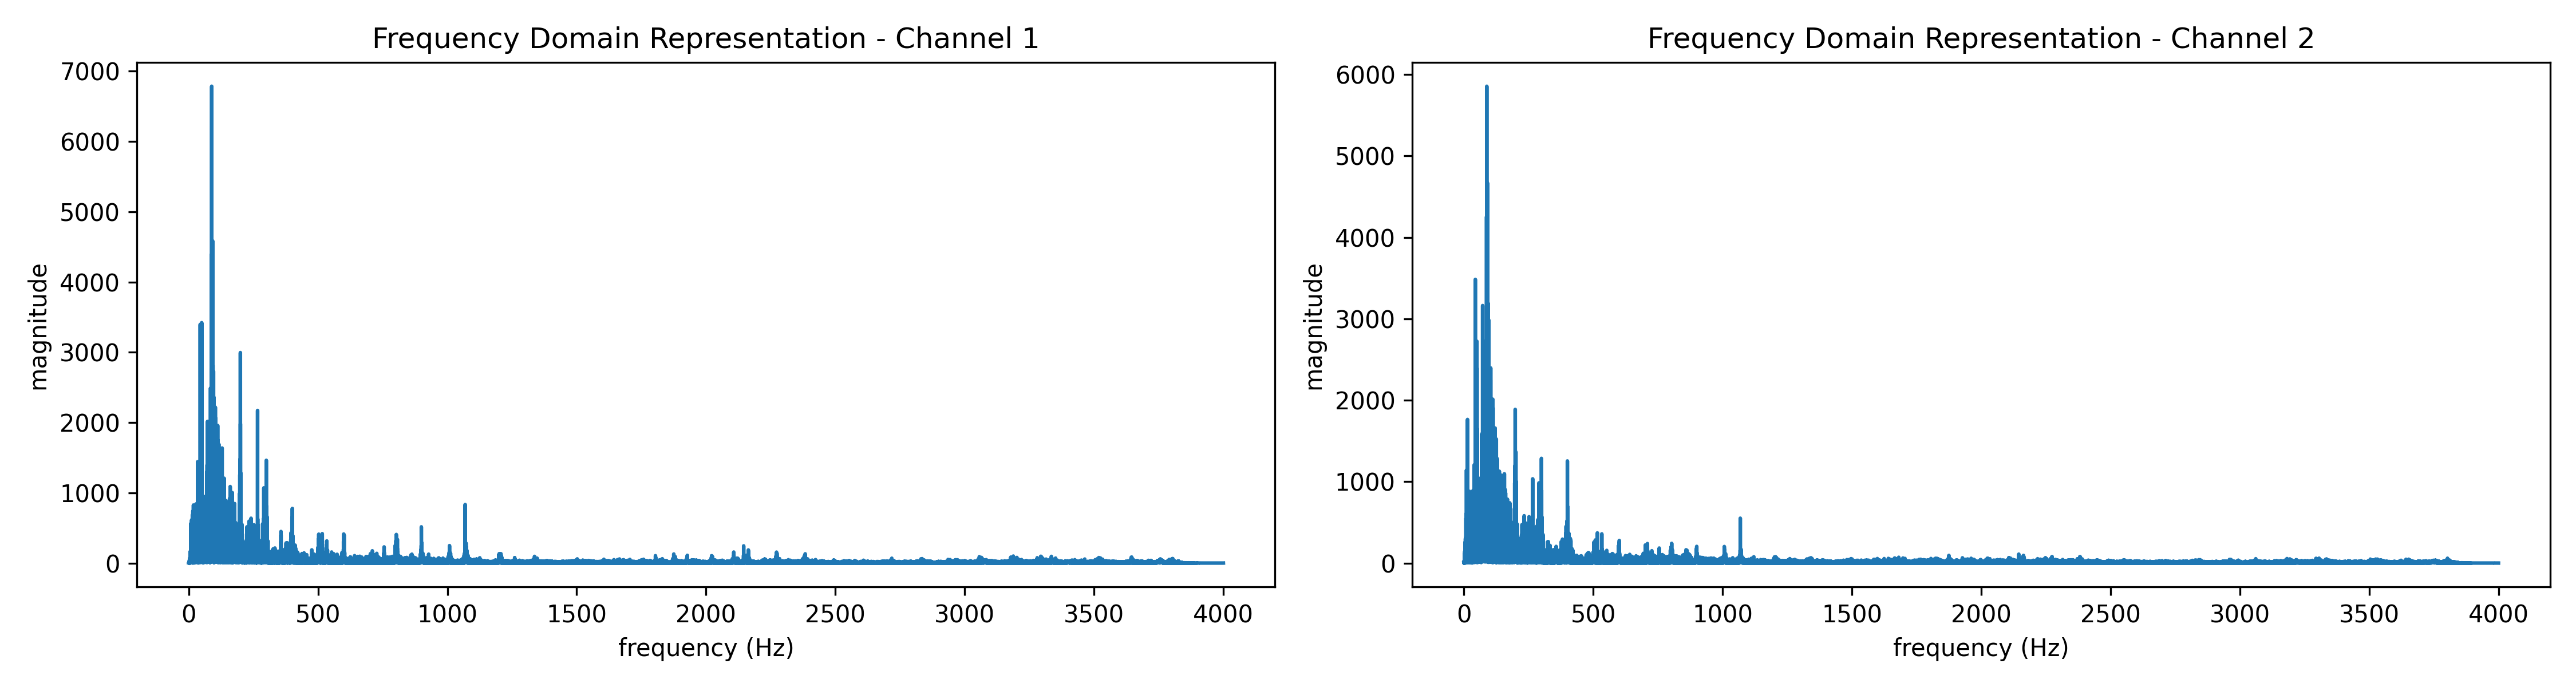
\includegraphics[width=\textwidth]{../Result/wav-frequency-domain-TX.png}
        \caption{Original}
        \label{fig:f-audio-linear-bsc-original}
    \end{subfigure}
    % \hfill
    \begin{subfigure}[b]{\textwidth}
        \centering
        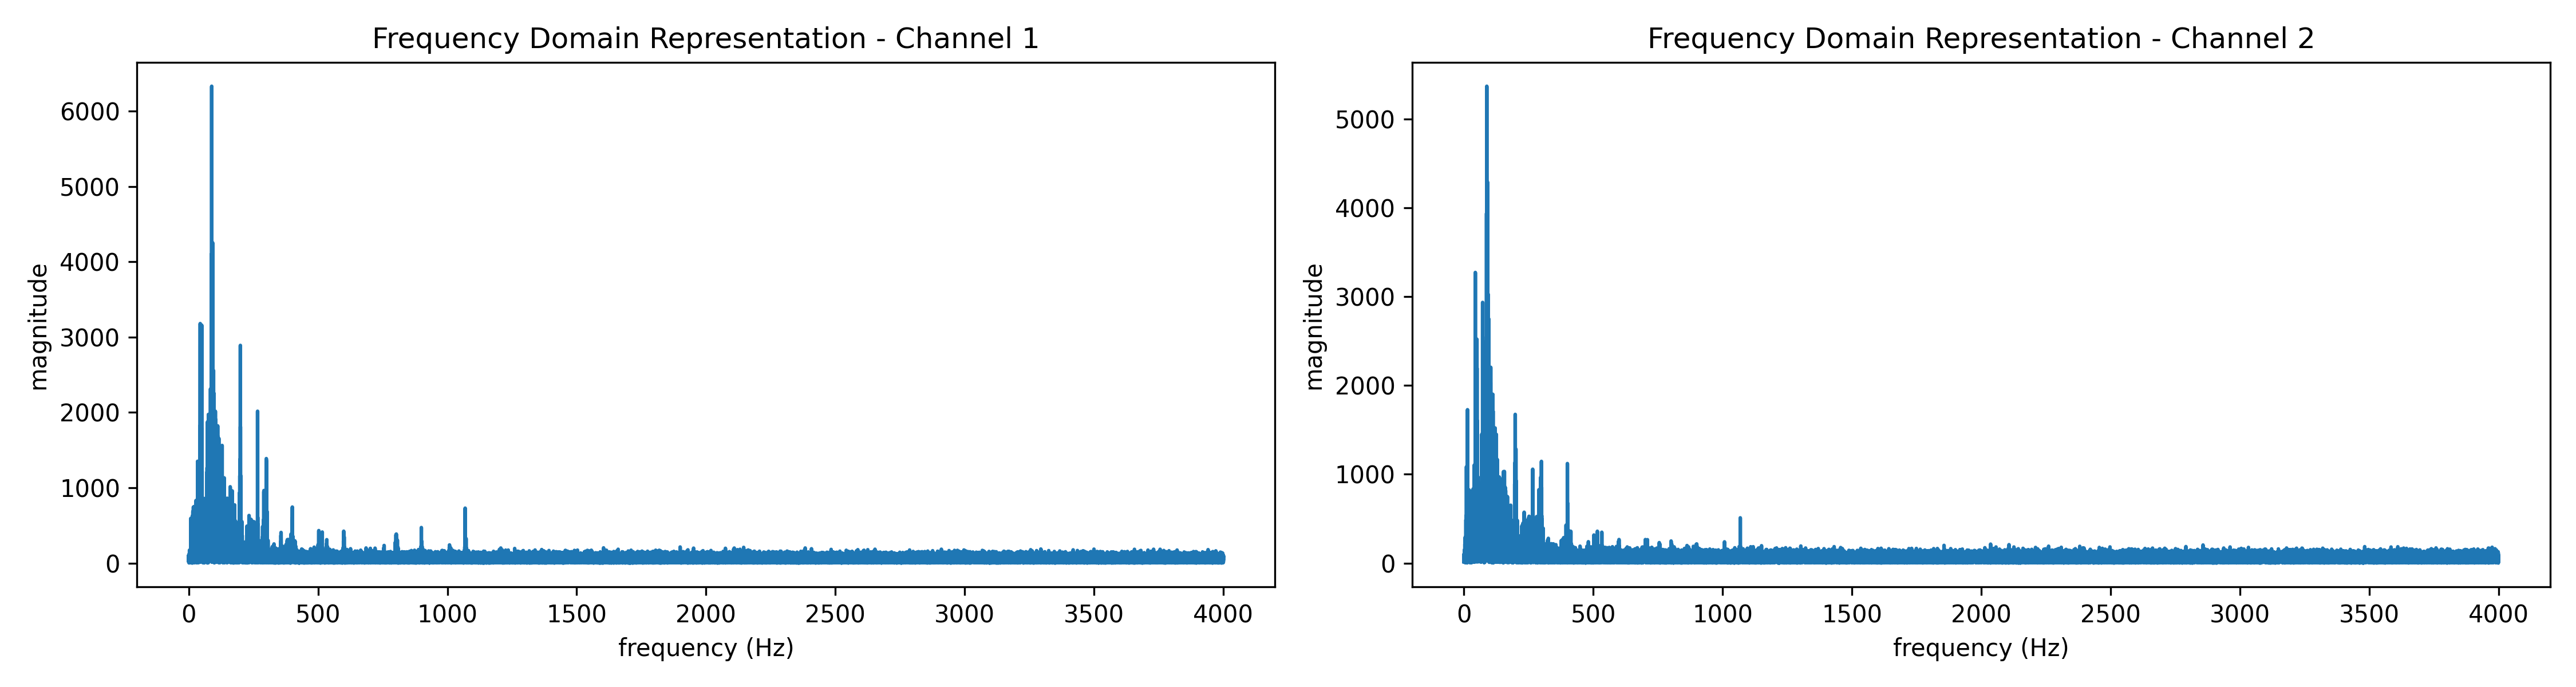
\includegraphics[width=\textwidth]{../Result/linear-bsc-wav-frequency-domain-RX.png}
        \caption{Without correction}
        \label{fig:f-audio-linear-bsc-no-correction}
    \end{subfigure}
    % \hfill
    \begin{subfigure}[b]{\textwidth}
        \centering
        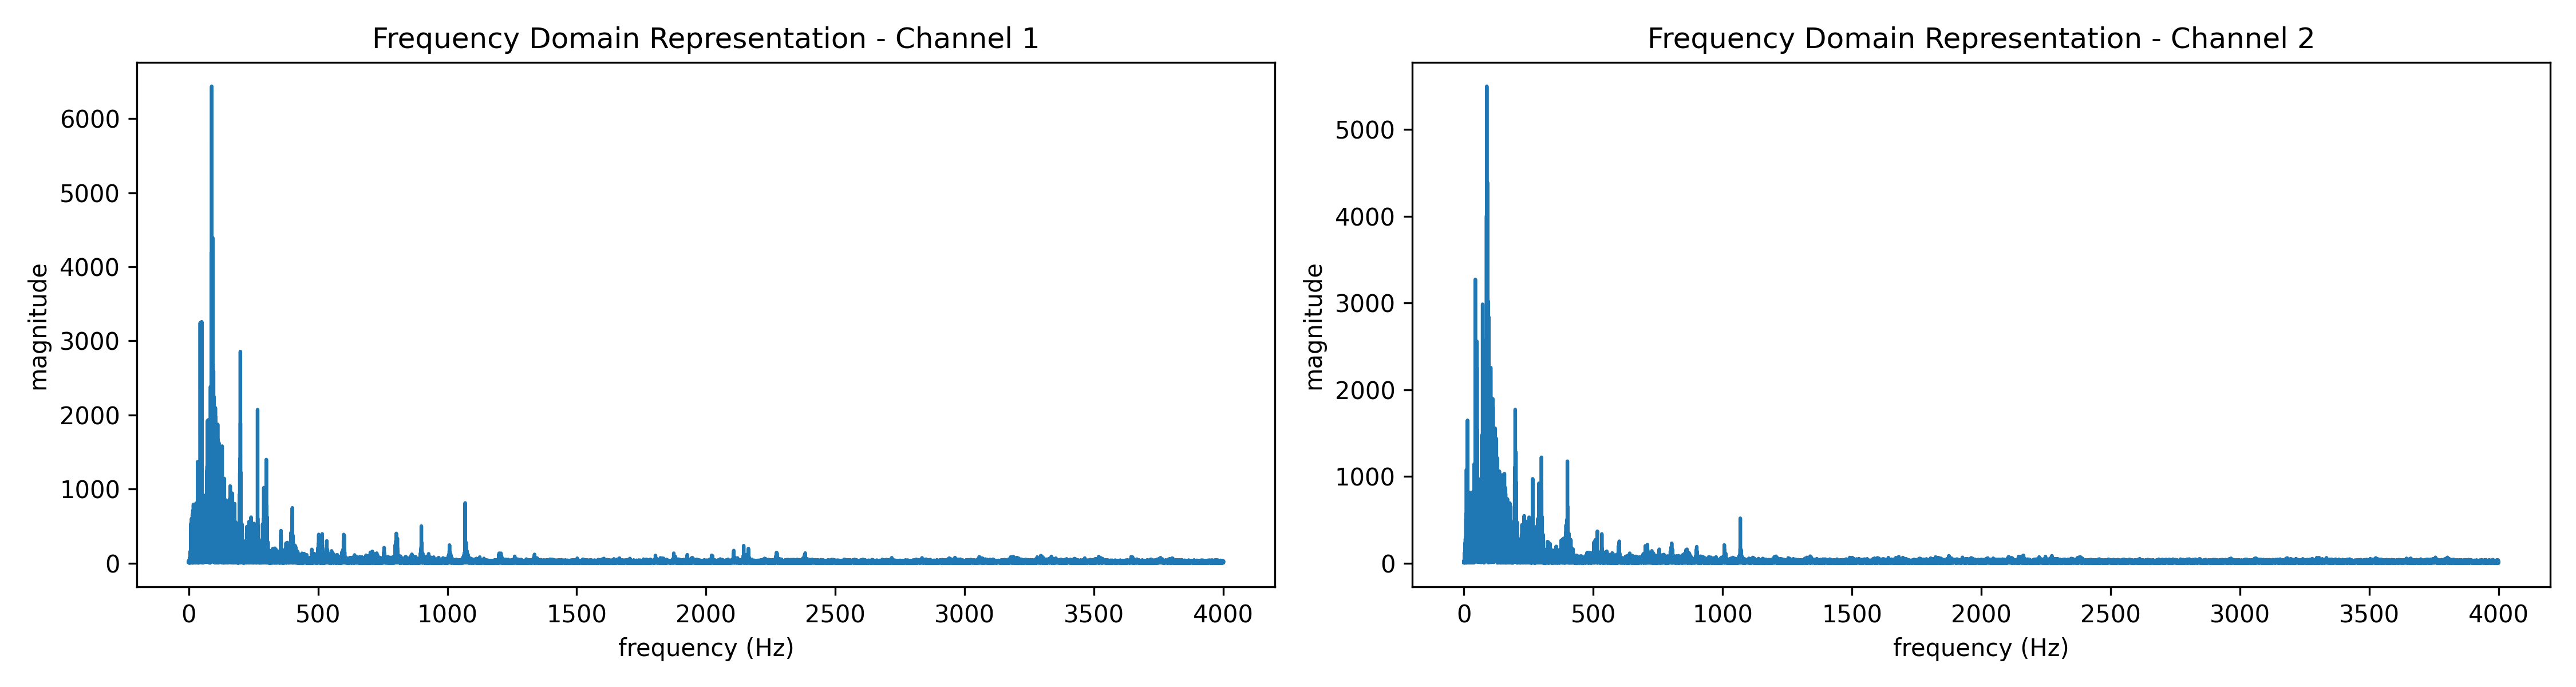
\includegraphics[width=\textwidth]{../Result/linear-bsc-wav-frequency-domain-RX-syndrome-corrected.png}
        \caption{Corrected}
        \label{fig:f-audio-linear-bsc-syndrome-corrected}
    \end{subfigure}
       \caption{Audio encoded with Linear Hamming passed through BSC}
       \label{fig:f-audio-linear-bsc}
\end{figure}


\section{$(n,k)$ Systematic Cyclic (Hamming) Code}
\subsection{Syndrome Decoder}
\subsubsection{Text string}

\begin{table}[htb]
    \centering
    \caption{Text string encoded with Cyclic Hamming passed through BSC}
    \label{tab:text-cyclic-bsc}
    \renewcommand{\arraystretch}{1.5}
    \begin{tabulary}{\textwidth}{ |L|L|L| } 
    \hline
    \textbf{Original} & \textbf{Without correction} & \textbf{Corrected} \\
    \hline
    Hello World! EEC269A Error Correcting Code Demo & H\textcolor{red}{u,}lo World! EEC269A Error Correcti\textcolor{red}{f}g Code Demo & Hello World! EEC269A Error Correcting Code Demo \\
    \hline
    \end{tabulary}
\end{table}



\subsubsection{Image}


\begin{figure}[htb]
    \centering
    \begin{subfigure}[b]{0.32\textwidth}
        \centering
        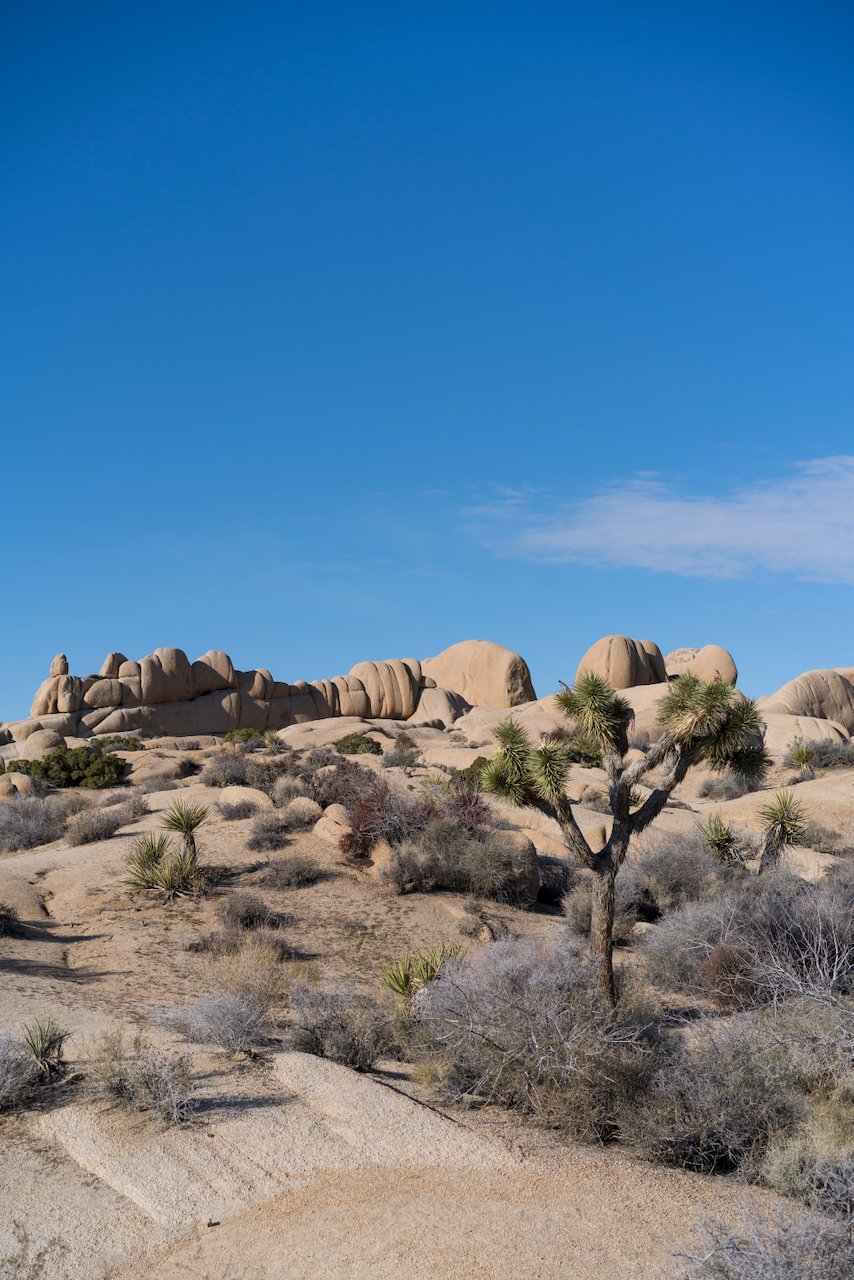
\includegraphics[width=\textwidth]{../Resource/image.png}
        \caption{Original}
        \label{fig:image-cyclic-bsc-original}
    \end{subfigure}
    \hfill
    \begin{subfigure}[b]{0.32\textwidth}
        \centering
        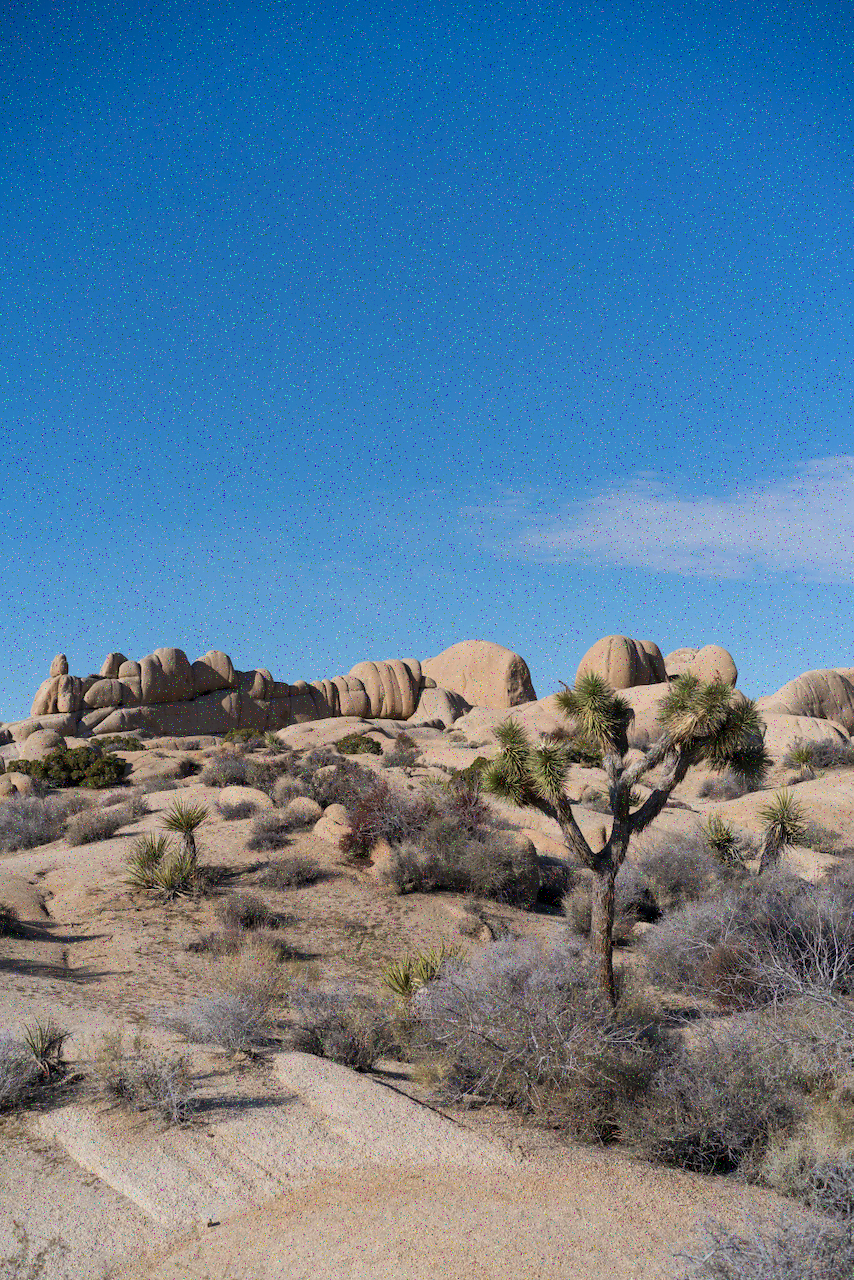
\includegraphics[width=\textwidth]{../Result/cyclic-bsc-output.png}
        \caption{Without correction}
        \label{fig:image-cyclic-bsc-no-correction}
    \end{subfigure}
    \hfill
    \begin{subfigure}[b]{0.32\textwidth}
        \centering
        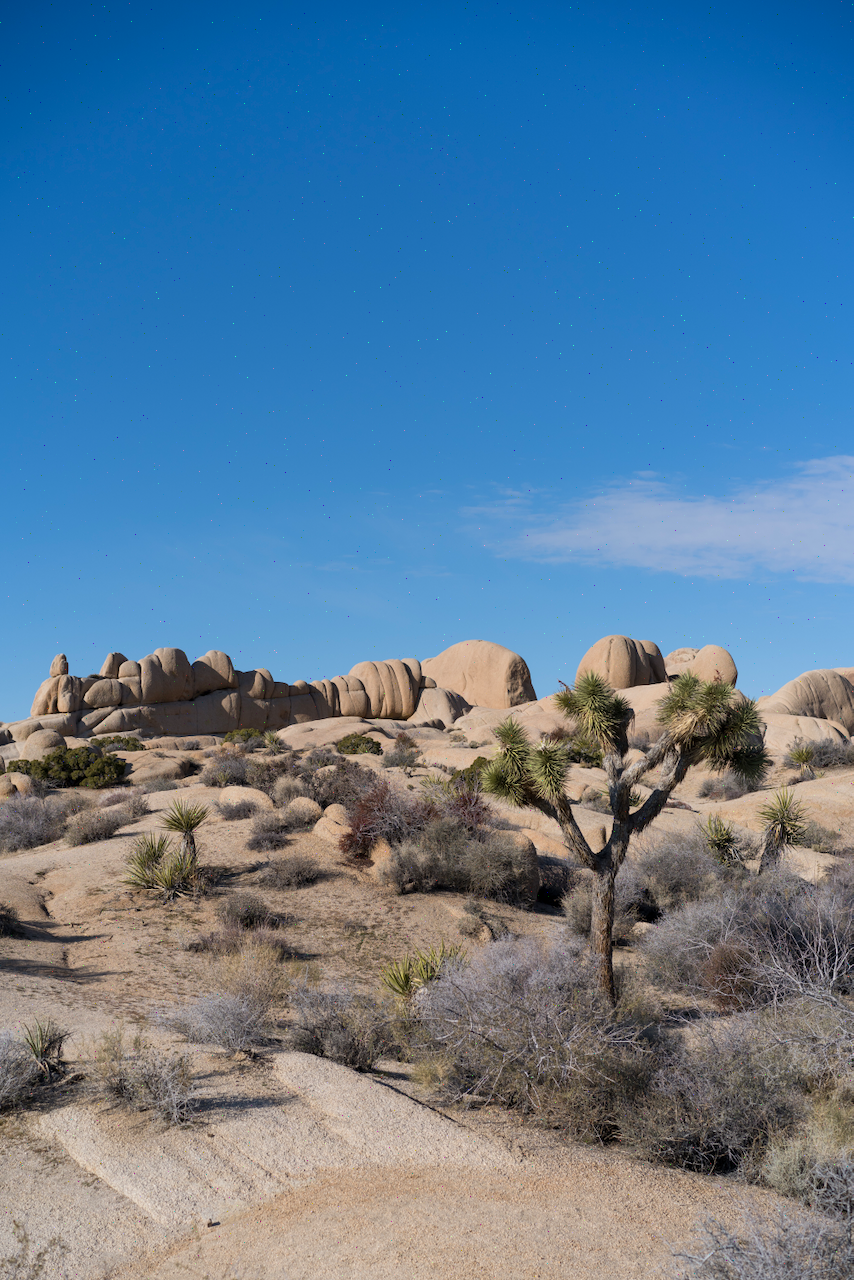
\includegraphics[width=\textwidth]{../Result/cyclic-bsc-output-syndrome-corrected.png}
        \caption{Corrected}
        \label{fig:image-cyclic-bsc-syndrome-corrected}
    \end{subfigure}
       \caption{Image encoded with Cyclic Hamming passed through BSC (entire)}
       \label{fig:image-cyclic-bsc}
\end{figure}




\begin{figure}[htb]
    \centering
    \begin{subfigure}[b]{0.32\textwidth}
        \centering
        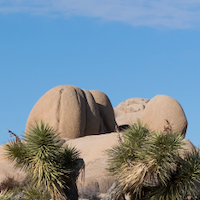
\includegraphics[width=\textwidth]{../Resource/cropped-image.png}
        \caption{Original}
        \label{fig:cropped-image-cyclic-bsc-original}
    \end{subfigure}
    \hfill
    \begin{subfigure}[b]{0.32\textwidth}
        \centering
        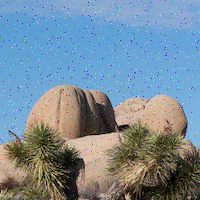
\includegraphics[width=\textwidth]{../Result/cropped-cyclic-bsc-output.png}
        \caption{Without correction}
        \label{fig:cropped-image-cyclic-bsc-no-correction}
    \end{subfigure}
    \hfill
    \begin{subfigure}[b]{0.32\textwidth}
        \centering
        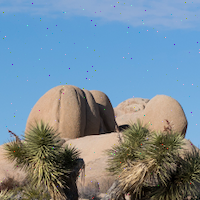
\includegraphics[width=\textwidth]{../Result/cropped-cyclic-bsc-output-syndrome-corrected.png}
        \caption{Corrected}
        \label{fig:cropped-image-cyclic-bsc-syndrome-corrected}
    \end{subfigure}
       \caption{Image encoded with Cyclic Hamming passed through BSC (details)}
       \label{fig:cropped-image-cyclic-bsc}
\end{figure}






\subsubsection{Audio}



\begin{figure}[htb]
    \centering
    \begin{subfigure}[b]{\textwidth}
        \centering
        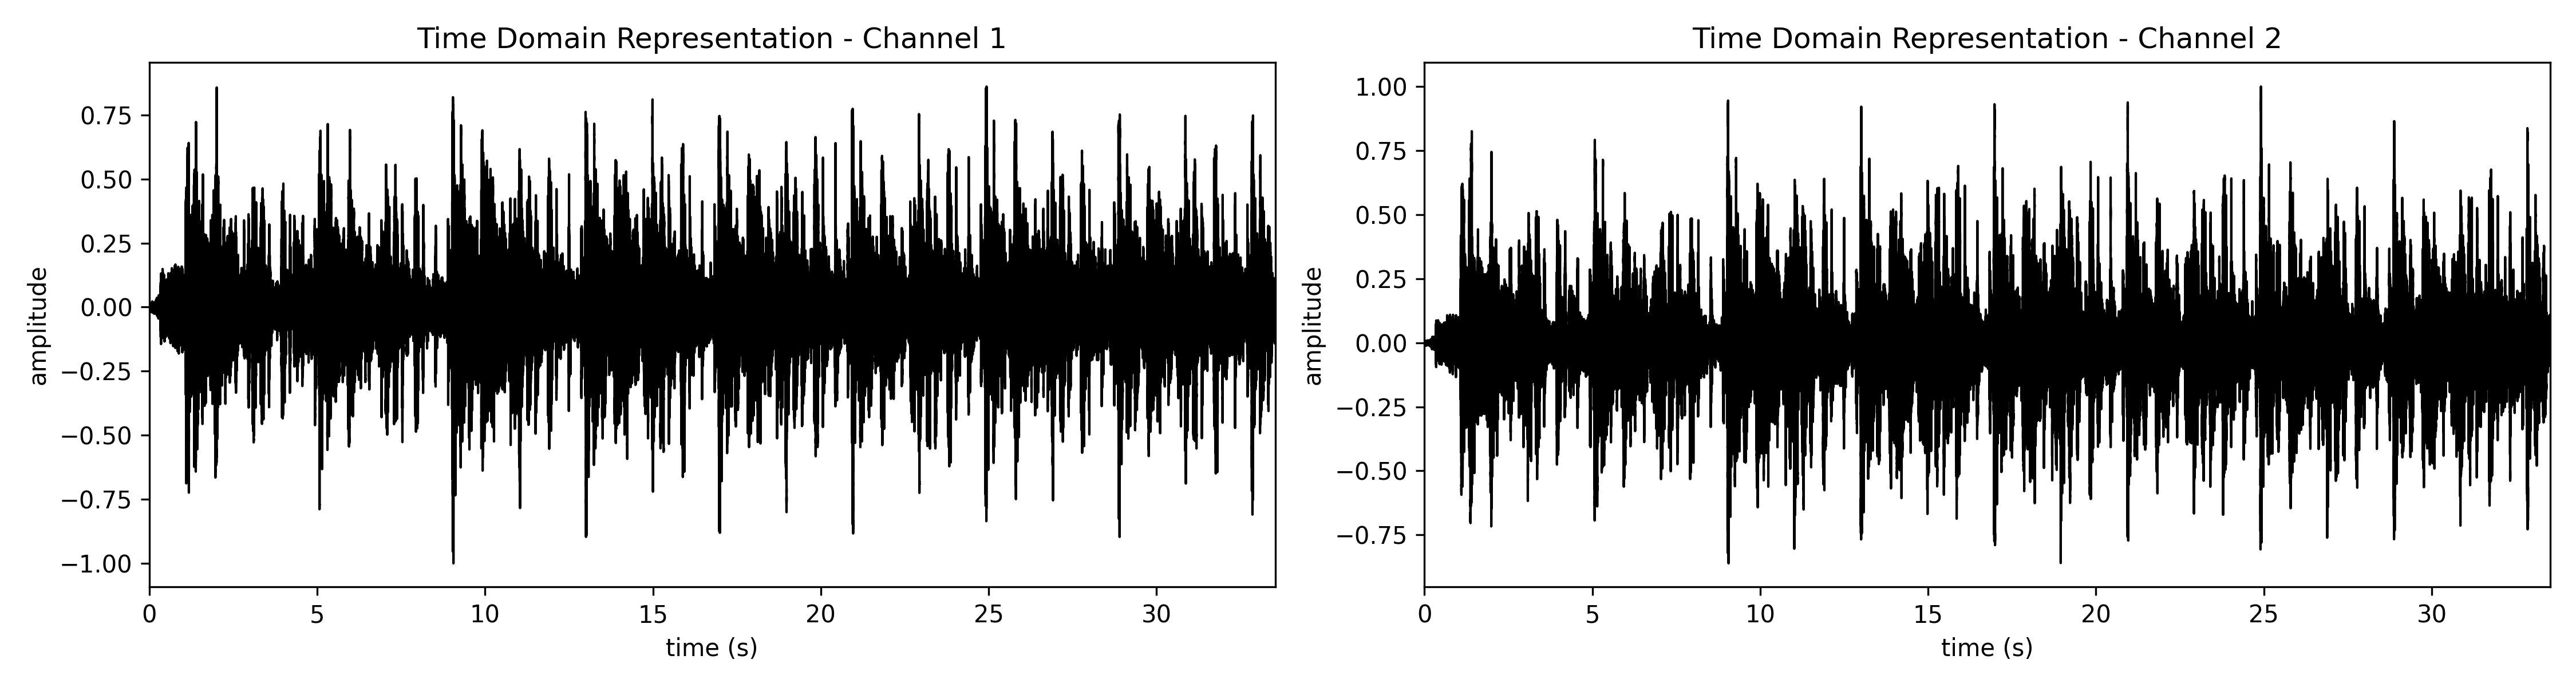
\includegraphics[width=\textwidth]{../Result/wav-time-domain-TX.png}
        \caption{Original}
        \label{fig:t-audio-cyclic-bsc-original}
    \end{subfigure}
    % \hfill
    \begin{subfigure}[b]{\textwidth}
        \centering
        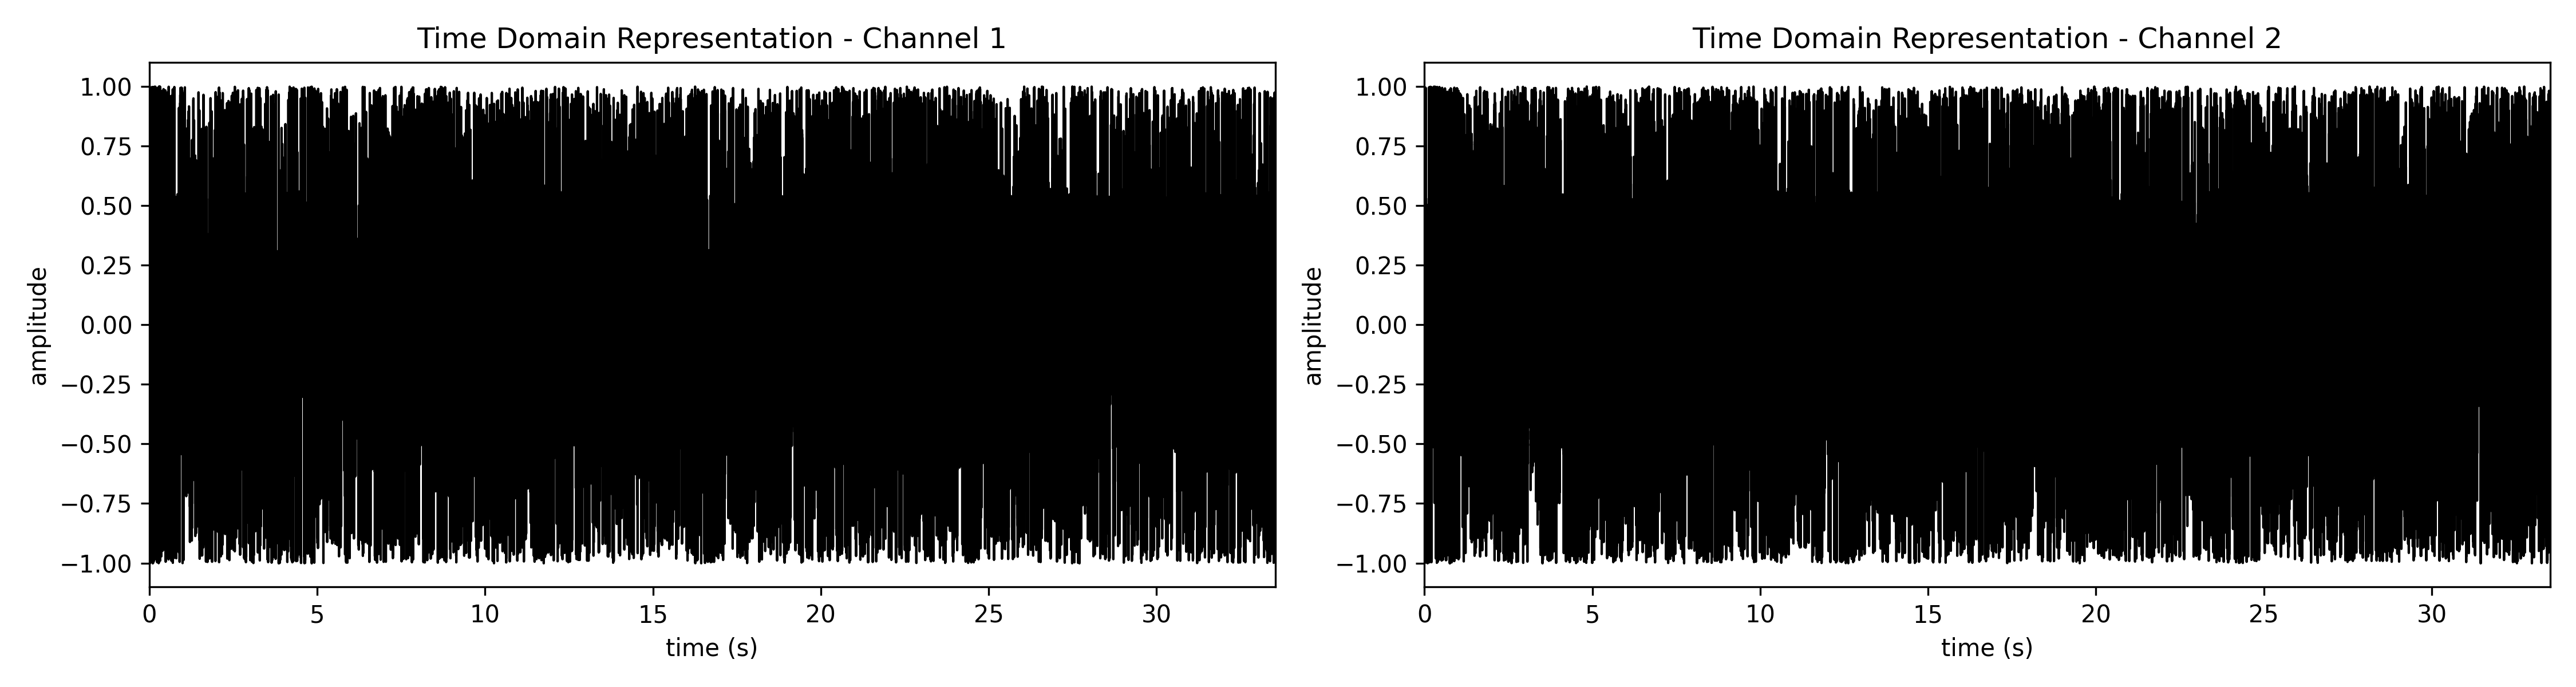
\includegraphics[width=\textwidth]{../Result/cyclic-bsc-wav-time-domain-RX.png}
        \caption{Without correction}
        \label{fig:t-audio-cyclic-bsc-no-correction}
    \end{subfigure}
    % \hfill
    \begin{subfigure}[b]{\textwidth}
        \centering
        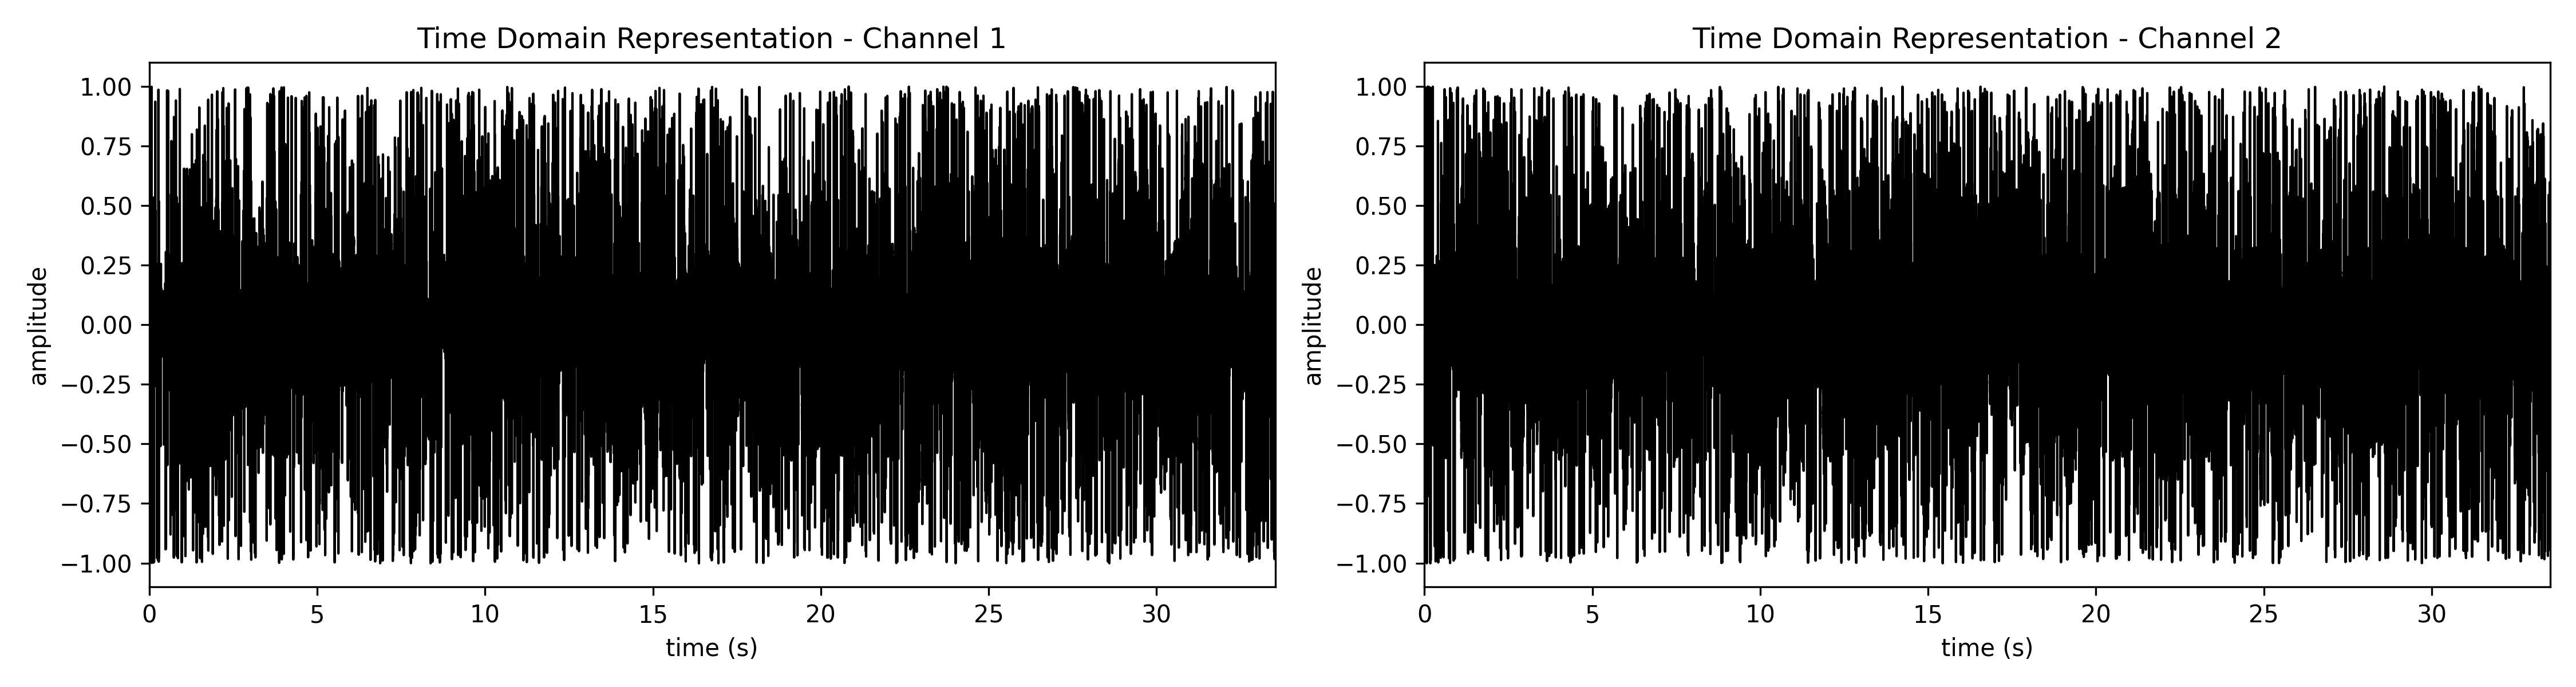
\includegraphics[width=\textwidth]{../Result/cyclic-bsc-wav-time-domain-RX-syndrome-corrected.png}
        \caption{Corrected}
        \label{fig:t-audio-cyclic-bsc-syndrome-syndrome-corrected}
    \end{subfigure}
       \caption{Audio encoded with Cyclic Hamming passed through BSC}
       \label{fig:t-audio-cyclic-bsc}
\end{figure}



\begin{figure}[htb]
    \centering
    \begin{subfigure}[b]{\textwidth}
        \centering
        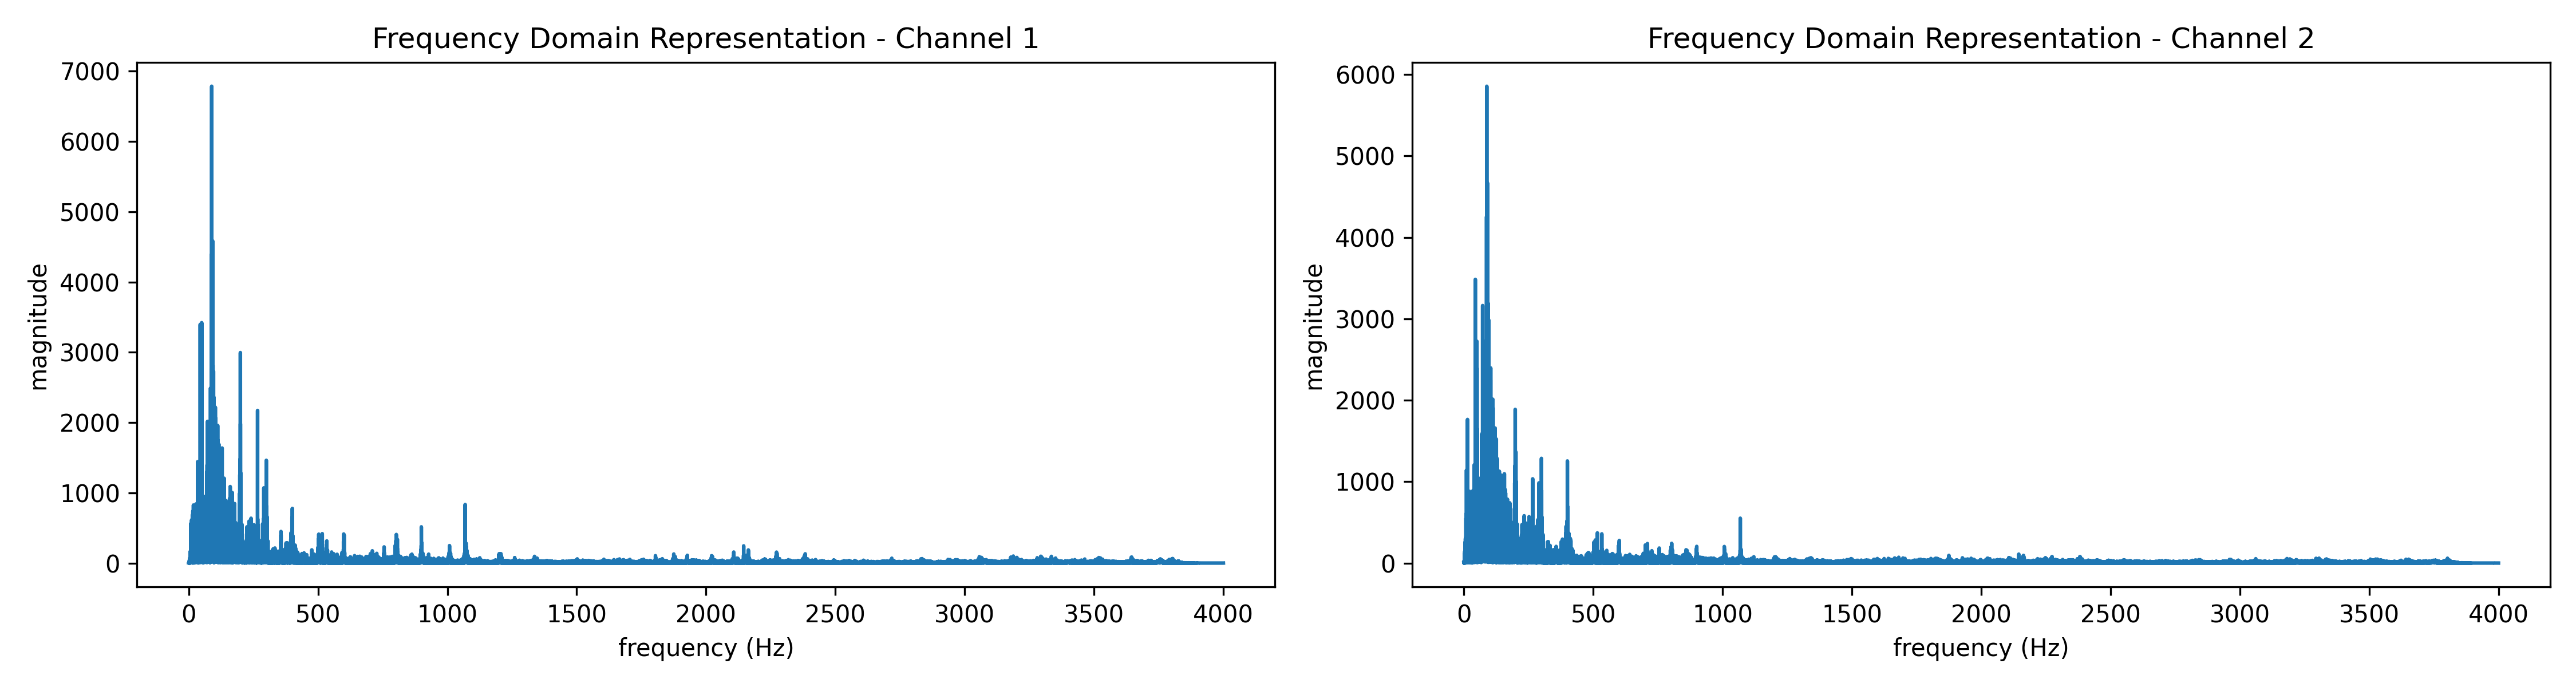
\includegraphics[width=\textwidth]{../Result/wav-frequency-domain-TX.png}
        \caption{Original}
        \label{fig:f-audio-cyclic-bsc-original}
    \end{subfigure}
    % \hfill
    \begin{subfigure}[b]{\textwidth}
        \centering
        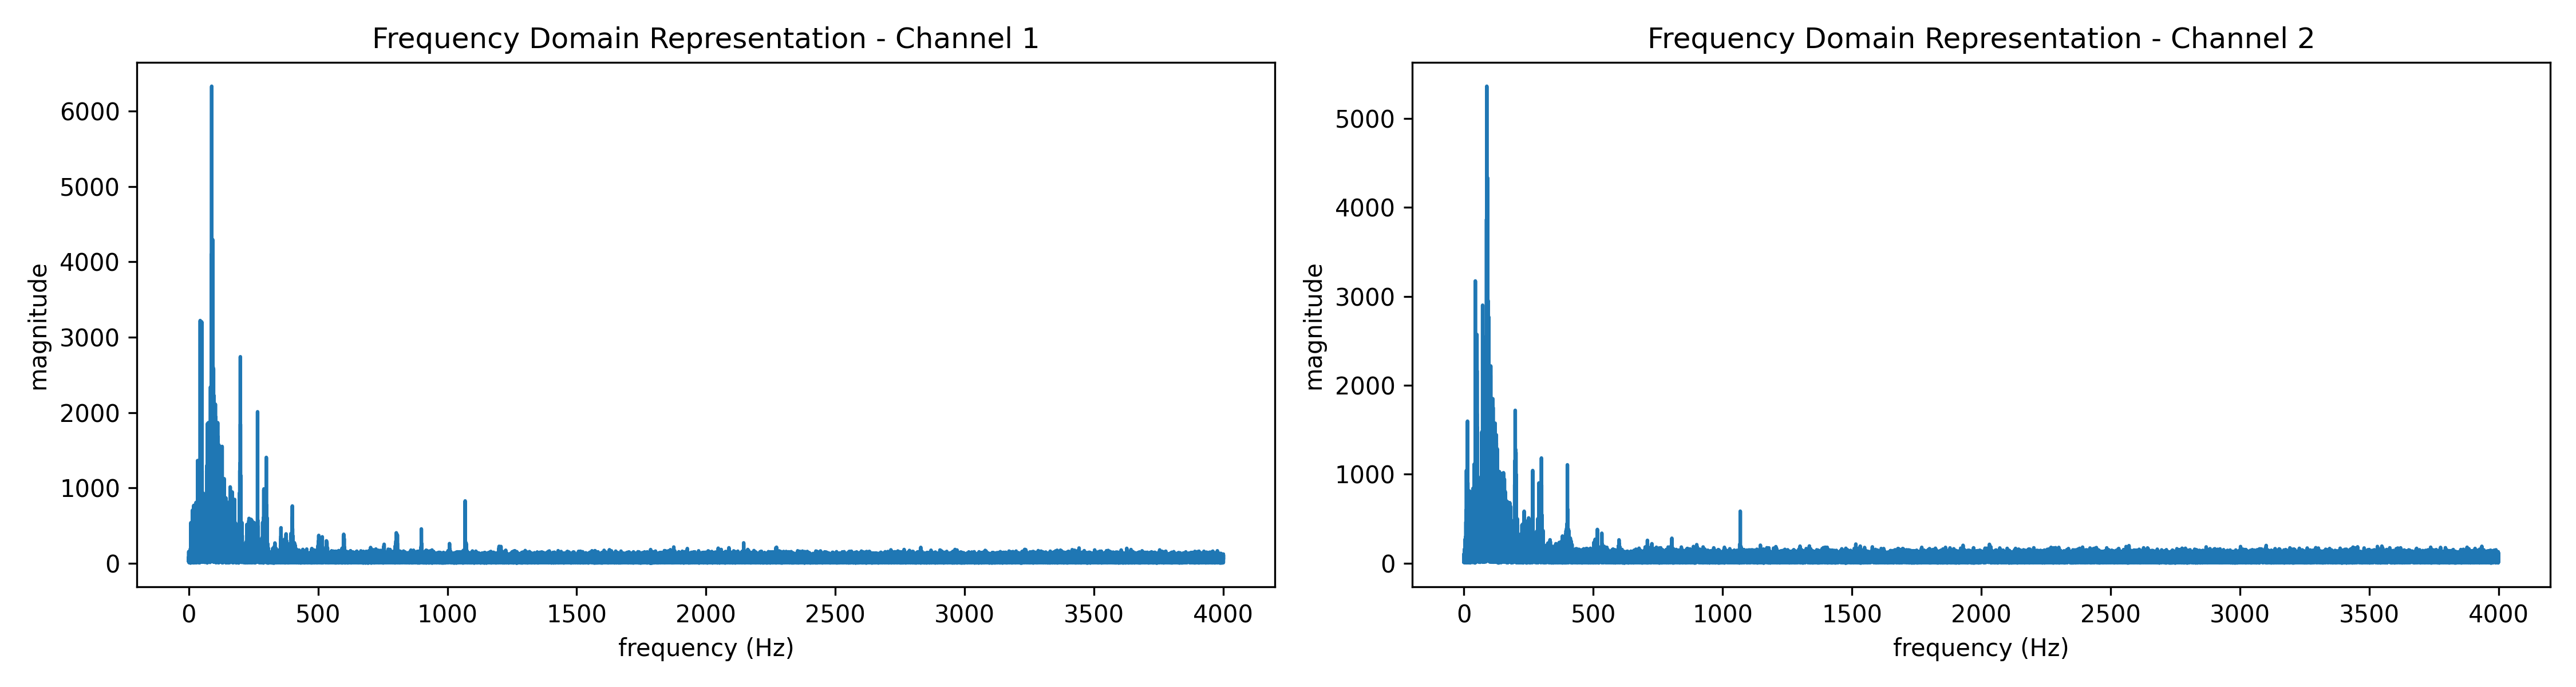
\includegraphics[width=\textwidth]{../Result/cyclic-bsc-wav-frequency-domain-RX.png}
        \caption{Without correction}
        \label{fig:f-audio-cyclic-bsc-no-correction}
    \end{subfigure}
    % \hfill
    \begin{subfigure}[b]{\textwidth}
        \centering
        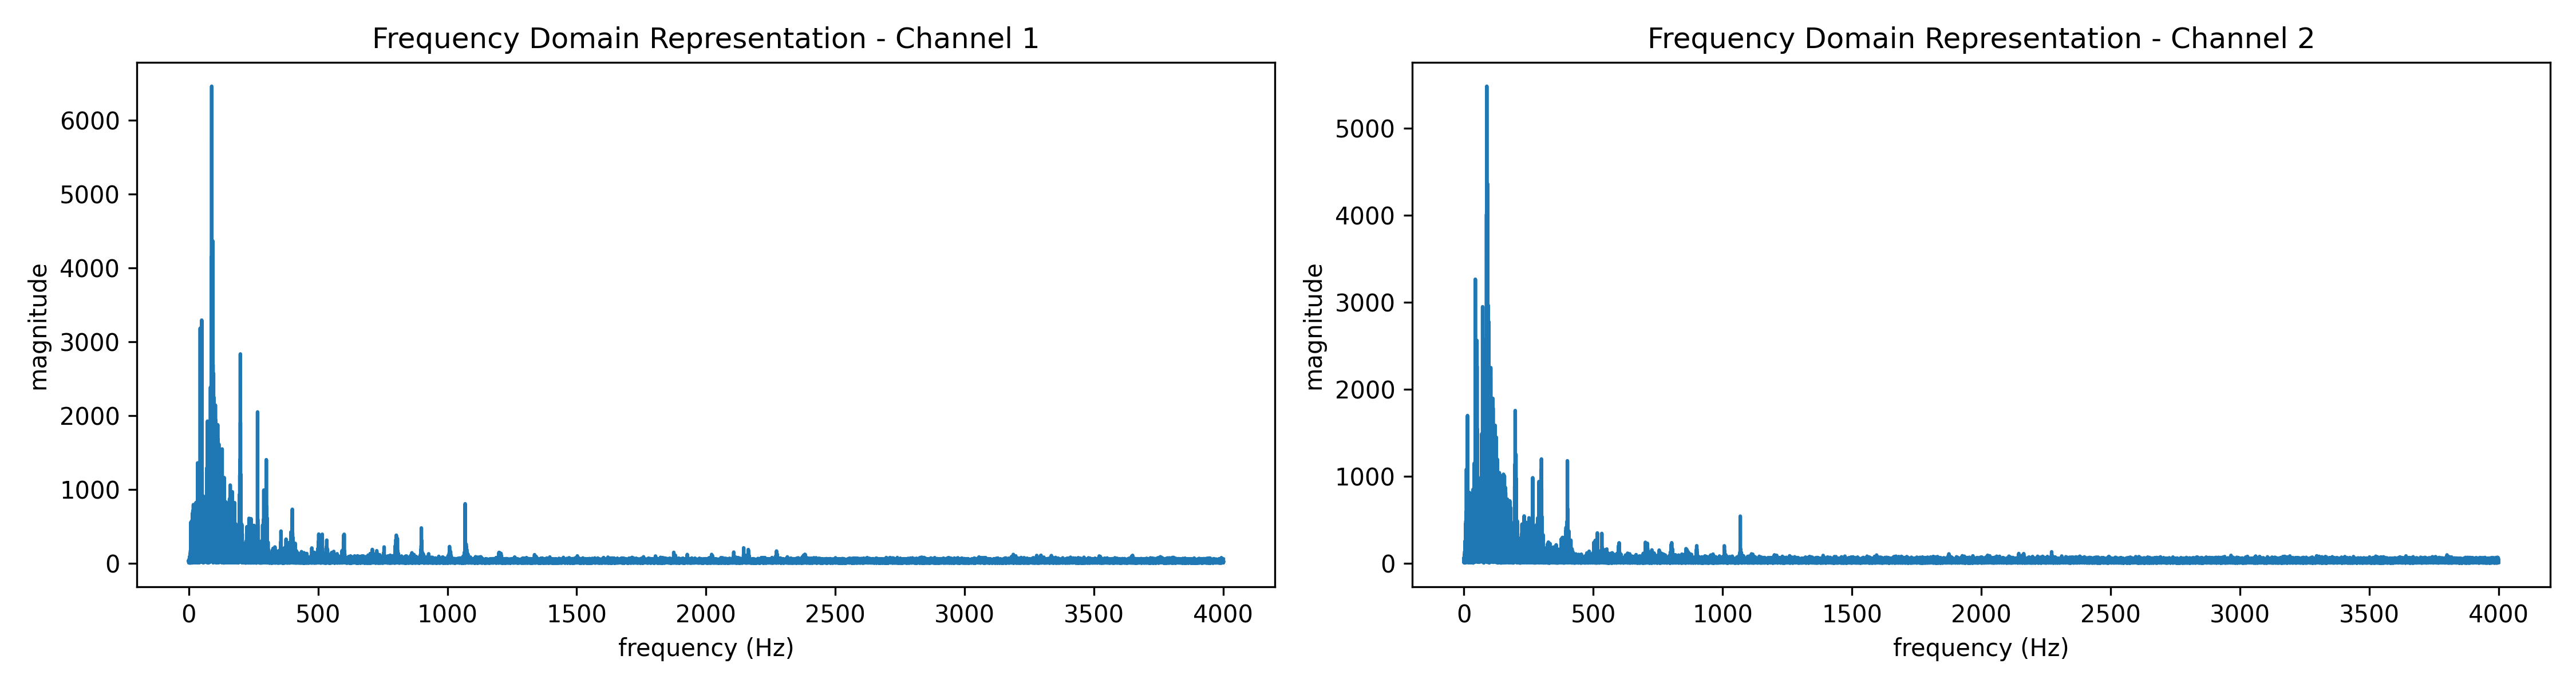
\includegraphics[width=\textwidth]{../Result/cyclic-bsc-wav-frequency-domain-RX-syndrome-corrected.png}
        \caption{Corrected}
        \label{fig:f-audio-cyclic-bsc-syndrome-corrected}
    \end{subfigure}
       \caption{Audio encoded with Cyclic Hamming passed through BSC}
       \label{fig:f-audio-cyclic-bsc}
\end{figure}






\subsection{LFSR Decoder}


\newpage
\section{Appendix: Python source code}
\subsection{Source}
\label{appendix:source}
\lstinputlisting[language=Python]{../Code/Source/source.py}

\subsection{Channel}
\label{appendix:channel}
\lstinputlisting[language=Python]{../Code/Channel/channel.py}

\subsection{Destination}
\label{appendix:destination}
\lstinputlisting[language=Python]{../Code/Destination/destination.py}

\subsection{Utilities}
\label{appendix:utils}
\lstinputlisting[language=Python]{../Code/Utils/plot_wav.py}
\lstinputlisting[language=Python]{../Code/Utils/polyTools.py}

\subsection{Linear code}
\label{appendix:linear-code}
\lstinputlisting[language=Python]{../Code/linear-code.py}

\subsection{Cyclic code}
\label{appendix:cyclic-code}
\lstinputlisting[language=Python]{../Code/cyclic-code.py}


\end{document}